%% thesis.tex 
%% Model LaTeX file for MEng/BEng thesis
%% School of Engineering, University of Edinburgh
%% v 1.0 2022-09 - First release
%% v 1.1 2022-11 - Added SAFE, IMFSE and LMP programmes
%% v 1.2 2023-11 - Minor corrections (typos) and clarifications
%% v 1.3 2024-06 - Added PhD in Engineering and added more content on figures, tables, mathematical expressions, and bibliography.
%% v 1.4 2025-03 - Added statement about permission to reuse thesis content and material


%% The following defines the document class used to structure and format your thesis. Do not change this.
\documentclass[11pt,twoside,openright]{report} 


%% The following are packages that are used by the template and that you will likely need for your content. Do not change this.

\usepackage[utf8]{inputenc}
% \usepackage{xunicode}
% \usepackage[english]{babel}
\usepackage[greek,english]{babel}
\usepackage{cmbright}
\usepackage{hologo}
% Use standard LaTeX citations instead of natbib for better compatibility
% \usepackage[numbers]{natbib}
% \citestyle{aysep={,}}
\usepackage{graphicx}
\usepackage{float}
\usepackage{setspace}
\usepackage{url}
\usepackage[nottoc]{tocbibind}
\usepackage{enumitem}
\usepackage{subcaption}

\usepackage{siunitx}
\usepackage{booktabs} % For professional quality tables
\usepackage{amsmath}  % For math symbols like \mathcal
\usepackage{bm}      % For bold math symbols like \bm{\delta}

%% Under this line, you can add additional packages that you may need for typesetting your document.

%\usepackage{...}


%%%%%%%%%%%%%%%%%%%%%%%%%%%%%%%%%%%%%%%%%%%%%%%%%%%%%%%%%%%%%%%%%%%%%%%%%%%%%%%%%%%%%%%%%%%%%%%%%%%%%%%%%%%%%%%%
%% The following defines some specific colours that is used in the text of this template (see section on table colouring).
\newcolumntype{G}{>{\centering\columncolor{blue!20!white}}p{0.2\textwidth}}



%%%%%%%%%%%%%%%%%%%%%%%%%%%%%%%%%%%%%%%%%%%%%%%%%%%%%%%%%%%%%%%%%%%%%%%%%%%%%%%%%%%%%%%%%%%%%%%%%%%%%%%%%%%%%%%%
%% The following says that all graphics (e.g. jpg, png, etc. files) will be searched in the "Figures/" folder. 
%% Do not change it, but ensure you indeed put your figures in that folder.

\graphicspath{{Figures/}}

%% Fix for Greek font encoding issues
\usepackage[T1]{fontenc}

%% Fix fancyhdr warning to speed up compilation
\setlength{\headheight}{28pt}


%%%%%%%%%%%%%%%%%%%%%%%%%%%%%%%%%%%%%%%%%%%%%%%%%%%%%%%%%%%%%%%%%%%%%%%%%%%%%%%%%%%%%%%%%%%%%%%%
%% Change \title, \author, \supervisor and \wordcount 
%% to your thesis title, your name., your supervisor's name and the word count of your thesis.
%% Do not touch \date.

\title{Solving Partial Integro-Differential Equations using Physics-Informed Neural Networks}

\author{Nikolaos Georgakopoulos}

\date{\the\year{}}

\newcommand{\supervisor}{[Prof/Dr] Supervisor Name}

%\newcommand{\wordcount}{1,000}


%%%%%%%%%%%%%%%%%%%%%%%%%%%%%%%%%%%%%%%%%%%%%%%%%%%%%%%%%%%%%%%%%%%%%%%%%%%%%%%%%%%%%%%%%%%%%%%%
%% The following loads the package UEDIN_SoE that has been setup specifically to format theses
%% of students in Civil and Environmental Engineering MEng/BEng programmes. 
%% In the line below, replace "mengSEWA" with any of the following:
%%   - "mengCE"    if you study on the "MEng Civil Engineering"
%%   - "bengCE"    if you study on the "BEng Civil Engineering"
%%   - "mengSAFE" if you study on the "MEng Structural and Fire Safety Engineering"
%%   - "bengSAFE" if you study on the "BEng Structural and Fire Safety Engineering"
%%   - "mengSEWA"  if you study on the "MEng Structural Engineering with Architecture"
%%   - "bengSEWA"  if you study on the "BEng Structural Engineering with Architecture"
%%   - "mscSAFE"  if you study on the "MSc in Structural and Fire Safety Engineering (SAFE)"
%%   - "mscFES"  if you study on the "MSc in Fire Engineering Science"
%%   - "mscIMFSE"  if you study on the "International Master of Science in Fire Safety Engineering (IMFSE)"
%%   - "mscLMP"  if you study on the "MSC Leading Major Programmes (LMP)"
%%   - "phdEng"  if you study on the "Doctor of Philosophy in Engineering"
\usepackage[mscAueb,fancyhdr,hyperref,colour]{UEDIN_SoE}

%% Configure PDF bookmarks to eliminate nesting appearance
\hypersetup{
    bookmarksdepth=1,        % Only show chapters in bookmarks (no sections)
    bookmarksopen=false,     % Don't auto-expand bookmarks
    bookmarksopenlevel=0,    % Start with everything collapsed
    pdfpagemode=UseNone,     % Don't show bookmarks panel by default
    hidelinks=true,          % Hide colored boxes around links
    pdfstartview=FitH        % Start with fit to page width
}

%% Define theorem environments (after UEDIN_SoE which loads amsthm)
\newtheorem{theorem}{Theorem}[chapter]
\newtheorem{lemma}[theorem]{Lemma}
\newtheorem{proposition}[theorem]{Proposition}
\newtheorem{corollary}[theorem]{Corollary}


%%%%%%%%%%%%%%%%%%%%%%%%%%%%%%%%%%%%%%%%%%%%%%%%%%%%%%%%%%%%%%%%%%%%%%%%%%%%%%%%%%%%%%%%%%%%%%%%%%
%%%%%%%%%%%%%%%%%%%%%%%%%%%%%%%%%%%%%%%%%%%%%%%%%%%%%%%%%%%%%%%%%%%%%%%%%%%%%%%%%%%%%%%%%%%%%%%%%%
\begin{document}

\doublespacing


%%%%%%%%%%%%%%%%%%%%%%%%%%%%%%%%%%%%%%%%%%%%%%%%%%%%%%%%%%%%%%%%%%%%%%%%%%%%%%%%%%%%%%%%%%%%%%%%%%
%% The following defines the title page and the frontmatter. 
%% To change the content of the frontmatter, go to "frontmatter.tex".

\maketitle

\pagenumbering{roman}

%%%%%%%%%%%%%%%%%%%%%%%%%%%%%%%%%%%%%%%%%%%%%%%%%%%%%%%%%%%%%%%%%%%%%%%%%%%%%%%%%%%%%%%%%%%%%%
%% This file contains the content for the frontmatter.
%%%%%%%%%%%%%%%%%%%%%%%%%%%%%%%%%%%%%%%%%%%%%%%%%%%%%%%%%%%%%%%%%%%%%%%%%%%%%%%%%%%%%%%%%%%%%%

%%%%%%%%%%%%%%%%%%%%%%%%%%%%%%%%%%%%%%%%%%%%%%%%%%%%%%%%%%%%%%%%%%%%%%%%%%%%%%%%%%%%%%%%%%%%%%
%% Declaration
%% Do not change this declaration section. However, read, check and accept its content

% \begin{declaration}{
%     This thesis is submitted in partial fulfilment of the requirements for the degree of \degreetext.
%     I declare that this thesis conforms to the University’s Academic Misconduct policies. 
%     It was composed by myself, the work contained therein is my own, except where explicitly stated otherwise in the text, and it has not been submitted, in whole or in part, for any other degree or professional qualification.
    
%     \vspace{0.5em} \noindent I hereby also grant my permission for this project to be stored, distributed and shown to other Athens University of Economics and Business students and staff for educational purposes.
% }\end{declaration}



%%%%%%%%%%%%%%%%%%%%%%%%%%%%%%%%%%%%%%%%%%%%%%%%%%%%%%%%%%%%%%%%%%%%%%%%%%%%%%%%%%%%%%%%%%%%%%
%% Abstract

\begin{abstract}
This thesis investigates the application of Physics-Informed Neural Networks (PINNs) to solve partial integro-differential equations (PIDEs) arising in financial mathematics, with particular focus on credit risk modeling. Traditional numerical methods for solving PIDEs, such as finite difference schemes, face computational challenges when dealing with jump-diffusion processes, especially in real-time applications requiring rapid probability of default calculations.

This work develops a comprehensive framework for approximating solutions to PIDEs governing Lévy-driven Ornstein-Uhlenbeck processes using deep neural networks. The methodology incorporates the governing equations directly into the neural network training process through a composite loss function that enforces the PIDE residual, boundary conditions, and terminal conditions simultaneously.

The experimental validation demonstrates that PINNs successfully learn accurate approximations of probability of default functions for jump-diffusion models. Comparison with Monte Carlo validates that the solution learnt by the PINN is indeed realistic. Most significantly, the trained PINN achieves computational speedups of over 3,600 times compared to traditional finite difference methods, reducing inference time from approximately 98 seconds to 0.027 seconds while maintaining comparable accuracy.

The results establish PINNs as a viable alternative to conventional numerical methods for solving financial PIDEs, particularly in scenarios requiring rapid evaluation across varying market conditions. The computational efficiency gains make sophisticated jump-diffusion models practically viable for real-time risk management applications, including algorithmic trading, portfolio optimization, and regulatory stress testing. This work contributes to the growing intersection of physics-informed machine learning and quantitative finance, demonstrating how modern deep learning techniques can address fundamental computational challenges in modelling dynamic systems governed by physical laws.
\end{abstract}


%%%%%%%%%%%%%%%%%%%%%%%%%%%%%%%%%%%%%%%%%%%%%%%%%%%%%%%%%%%%%%%%%%%%%%%%%%%%%%%%%%%%%%%%%%%%%%
%% Greek Abstract

% \begin{abstract}
% \selectlanguage{greek}
% % % \textbf{Περίληψη}

% Αυτή η διπλωματική εργασία διερευνά την εφαρμογή των Φυσικά Ενημερωμένων Νευρωνικών Δικτύων (Physics-Informed Neural Networks - PINNs) για την επίλυση μερικών ολοκληρο-διαφορικών εξισώσεων (PIDEs) που προκύπτουν στα χρηματοοικονομικά μαθηματικά, με ιδιαίτερη εστίαση στη μοντελοποίηση πιστωτικού κινδύνου. Οι παραδοσιακές αριθμητικές μέθοδοι για την επίλυση PIDEs, όπως τα σχήματα πεπερασμένων διαφορών, αντιμετωπίζουν υπολογιστικές προκλήσεις όταν ασχολούνται με διαδικασίες άλματος-διάχυσης, ειδικά σε εφαρμογές πραγματικού χρόνου που απαιτούν ταχείς υπολογισμούς πιθανότητας αθέτησης.

% % % Η εργασία αυτή αναπτύσσει ένα ολοκληρωμένο πλαίσιο για την προσέγγιση λύσεων σε PIDEs που διέπουν διαδικασίες Ornstein-Uhlenbeck οδηγούμενες από Lévy χρησιμοποιώντας βαθιά νευρωνικά δίκτυα. Η μεθοδολογία ενσωματώνει τις κυβερνητικές εξισώσεις απευθείας στη διαδικασία εκπαίδευσης του νευρωνικού δικτύου μέσω μιας σύνθετης συνάρτησης απώλειας που επιβάλλει ταυτόχρονα το υπόλοιπο της PIDE, τις συνοριακές συνθήκες και τις τελικές συνθήκες.

% % % Η πειραματική επικύρωση δείχνει ότι τα PINNs μαθαίνουν επιτυχώς ακριβείς προσεγγίσεις των συναρτήσεων πιθανότητας αθέτησης για μοντέλα άλματος-διάχυσης. Η σύγκριση με προσομοιώσεις Monte Carlo επικυρώνει ότι η λύση που μαθαίνει το PINN είναι πραγματικά ρεαλιστική. Το σημαντικότερο είναι ότι το εκπαιδευμένο PINN επιτυγχάνει υπολογιστικές επιταχύνσεις άνω των 3.600 φορών σε σύγκριση με τις παραδοσιακές μεθόδους πεπερασμένων διαφορών, μειώνοντας τον χρόνο συμπερασμού από περίπου 98 δευτερόλεπτα σε 0.027 δευτερόλεπτα διατηρώντας παρόμοια ακρίβεια.

% % % Τα αποτελέσματα καθιστούν τα PINNs ως μια βιώσιμη εναλλακτική λύση στις συμβατικές αριθμητικές μεθόδους για την επίλυση χρηματοοικονομικών PIDEs, ιδιαίτερα σε σενάρια που απαιτούν ταχεία αξιολόγηση σε διαφορετικές συνθήκες αγοράς. Τα οφέλη υπολογιστικής απόδοσης καθιστούν τα εξελιγμένα μοντέλα άλματος-διάχυσης πρακτικά βιώσιμα για εφαρμογές διαχείρισης κινδύνου σε πραγματικό χρόνο, συμπεριλαμβανομένων των αλγοριθμικών συναλλαγών, της βελτιστοποίησης χαρτοφυλακίου και των ρυθμιστικών δοκιμών αντοχής. Αυτή η εργασία συμβάλλει στην αυξανόμενη τομή της φυσικά ενημερωμένης μηχανικής μάθησης και των ποσοτικών χρηματοοικονομικών, αποδεικνύοντας πώς οι σύγχρονες τεχνικές βαθιάς μάθησης μπορούν να αντιμετωπίσουν θεμελιώδεις υπολογιστικές προκλήσεις στη μοντελοποίηση δυναμικών συστημάτων που διέπονται από φυσικούς νόμους.
% \selectlanguage{english}
% \end{abstract}

% Define the Greek abstract environment
% \newenvironment{greekabstract}
%     {\chapter*{Greek Abstract}\addcontentsline{toc}{chapter}{Greek Abstract}}
   

% Greek Abstract
\begin{greekabstract}
    \selectlanguage{greek}
    Αυτή η διπλωματική εργασία διερευνά την εφαρμογή των Φυσικά Ενημερωμένων Νευρωνικών Δικτύων (\selectlanguage{english}Physics-Informed Neural Networks - PINNs\selectlanguage{greek}) για την επίλυση μερικών ολοκληρο-διαφορικών εξισώσεων (\selectlanguage{english}PIDEs\selectlanguage{greek}) που προκύπτουν στα χρηματοοικονομικά μαθηματικά, με ιδιαίτερη εστίαση στη μοντελοποίηση πιστωτικού κινδύνου. Οι παραδοσιακές αριθμητικές μέθοδοι για την επίλυση \selectlanguage{english}PIDEs\selectlanguage{greek}, όπως τα σχήματα πεπερασμένων διαφορών, αντιμετωπίζουν υπολογιστικές προκλήσεις όταν ασχολούνται με διαδικασίες άλματος-διάχυσης, ειδικά σε εφαρμογές πραγματικού χρόνου που απαιτούν γρήγορους υπολογισμούς πιθανότητας αθέτησης.

    Η εργασία αυτή αναπτύσσει ένα ολοκληρωμένο πλαίσιο για την προσέγγιση λύσεων σε \selectlanguage{english}PIDEs\selectlanguage{greek} που διέπουν τις διαδικασίες \selectlanguage{english}Ornstein-Uhlenbeck\selectlanguage{greek} οδηγούμενες από διαδικασίες\selectlanguage{english}Lévy\selectlanguage{greek} χρησιμοποιώντας βαθιά νευρωνικά δίκτυα. Η μεθοδολογία ενσωματώνει τις εξισώσεις που υπαγορεύουν τις εν λόγω διαδικασίες, απευθείας στη διαδικασία εκπαίδευσης του νευρωνικού δικτύου μέσω μιας σύνθετης συνάρτησης κόστους που επιβάλλει ταυτόχρονα το υπόλοιπο της \selectlanguage{english}PIDE\selectlanguage{greek}, τις συνοριακές συνθήκες και τις τελικές συνθήκες.
    
    Η πειραματική αξιολόγηση δείχνει ότι τα \selectlanguage{english}PINNs\selectlanguage{greek} μαθαίνουν επιτυχώς ακριβείς προσεγγίσεις των συναρτήσεων πιθανότητας αθέτησης για μοντέλα άλματος-διάχυσης. Η σύγκριση με προσομοιώσεις \selectlanguage{english}Monte Carlo\selectlanguage{greek} επικυρώνει ότι η λύση που μαθαίνει το \selectlanguage{english}PINN\selectlanguage{greek} είναι πραγματικά ρεαλιστική. Το σημαντικότερο είναι ότι το εκπαιδευμένο \selectlanguage{english}PINN\selectlanguage{greek} επιτυγχάνει υπολογιστικές επιταχύνσεις άνω των 3.600 φορών σε σύγκριση με τις παραδοσιακές μεθόδους πεπερασμένων διαφορών, μειώνοντας τον χρόνο υπολογισμού της λύσης από περίπου 98 δευτερόλεπτα σε 0.027 δευτερόλεπτα διατηρώντας παρόμοια ακρίβεια.
    
    Τα αποτελέσματα καθιστούν τα \selectlanguage{english}PINNs\selectlanguage{greek} ως μια βιώσιμη εναλλακτική λύση στις συμβατικές αριθμητικές μεθόδους για την επίλυση χρηματοοικονομικών \selectlanguage{english}PIDEs\selectlanguage{greek}, ιδιαίτερα σε σενάρια που απαιτούν ταχεία αξιολόγηση σε διαφορετικές συνθήκες αγοράς. Τα οφέλη υπολογιστικής απόδοσης καθιστούν τα εξελιγμένα μοντέλα άλματος-διάχυσης πρακτικά βιώσιμα για εφαρμογές διαχείρισης κινδύνου σε πραγματικό χρόνο, συμπεριλαμβανομένων των αλγοριθμικών συναλλαγών, της βελτιστοποίησης χαρτοφυλακίου και των ρυθμιστικών δοκιμών αντοχής. Αυτή η εργασία συμβάλλει στην αυξανόμενη τομή της φυσικά ενημερωμένης μηχανικής μάθησης και των ποσοτικών χρηματοοικονομικών, αποδεικνύοντας πώς οι σύγχρονες τεχνικές βαθιάς μάθησης μπορούν να αντιμετωπίσουν θεμελιώδεις υπολογιστικές προκλήσεις στη μοντελοποίηση δυναμικών συστημάτων που διέπονται από φυσικούς νόμους.
{\selectlanguage{english}}

\end{greekabstract}

%%%%%%%%%%%%%%%%%%%%%%%%%%%%%%%%%%%%%%%%%%%%%%%%%%%%%%%%%%%%%%%%%%%%%%%%%%%%%%%%%%%%%%%%%%%%%%
%% Dedication

\begin{acknowledgements}
    I would like to thank my family and friends for their support during my master's studies and the completion of this thesis. Furthermore, I would like to extend gratitude to my supervisors K. Georgiou and AN Yannacopoulos for their support, mentorship and kindness.
    
    \vspace{1cm}
    
    In the spirit of open, transparent, and reproducible science, I have made all code, models, and data for this thesis publicly available at: \url{https://github.com/ngeorgakop/levy_ou_pinn}
\end{acknowledgements}


%%%%%%%%%%%%%%%%%%%%%%%%%%%%%%%%%%%%%%%%%%%%%%%%%%%%%%%%%%%%%%%%%%%%%%%%%%%%%%%%%%%%%%%%%%%%%%
%% Tables of Content, Figures and Tables

\tableofcontents

\listoffigures

\listoftables


%%%%%%%%%%%%%%%%%%%%%%%%%%%%%%%%%%%%%%%%%%%%%%%%%%%%%%%%%%%%%%%%%%%%%%%%%%%%%%%%%%%%%%%%%%%%%%
%% Glossary - Abbreviations
%% Do not alter the content below (the content for those is defined in definitions.tex

% \chapter*{Abbreviations}
% \addcontentsline{toc}{chapter}{Abbrevations}
% % Acronyms on its first use see after ToCs
% \glsunsetall % Disable all
% % Show all regardless if they are used or not (if that is what you want).
% \glsaddall
% \glsaddallunused
% \setglossarysection{section}
% \printglossary[type=\acronymtype,title={}]
% \paragraph{Note:} Author abbreviations are shown in their corresponding reference entry.

% \setlength{\glsdescwidth}{0.5\textwidth}
% \setlength{\glspagelistwidth}{0.1\textwidth}
% \cleardoublepage


%%%%%%%%%%%%%%%%%%%%%%%%%%%%%%%%%%%%%%%%%%%%%%%%%%%%%%%%%%%%%%%%%%%%%%%%%%%%%%%%%%%%%%%%%%%%%%
%% Glossary - Nomenclature
%% Do not alter the content below (the content for those is defined in definitions.tex

% \chapter*{Nomenclature}
% \addcontentsline{toc}{chapter}{Nomenclature}
% \setglossarysection{section}
% \glossarystyle{aiaostyle}
% \printglossary[type=main,title={}]
% \vspace{1cm}
% \glossarystyle{nounits}
% % \paragraph{Note:} Other terms are introduced as they are presented in the studies.

% % Enable entries again
% \glsresetall

% \cleardoublepage


\pagenumbering{arabic}



%%%%%%%%%%%%%%%%%%%%%%%%%%%%%%%%%%%%%%%%%%%%%%%%%%%%%%%%%%%%%%%%%%%%%%%%%%%%%%%%%%%%%%%%%%%%%%%%%%
%% The main content starts here.

\chapter{Introduction}
\label{chap:intro_levy_credit}

\section{Introduction and Motivation for Advanced Stochastic Models in Credit Risk}
\label{sec:intro_chapter1}

The mathematical modeling of financial systems has evolved significantly since Bachelier's early use of Brownian motion to describe price fluctuations \cite{bachelier1900theorie}. While diffusion-based models, such as those underlying the Black-Scholes-Merton framework, have been foundational in quantitative finance, their reliance on continuous sample paths limits their ability to capture the sudden, discontinuous events observed in real-world credit risk—such as unexpected defaults or abrupt changes in credit spreads.

Structural credit risk models, beginning with Merton's approach, typically assume a firm's asset value follows a Geometric Brownian Motion (GBM) \cite{merton1974pricing}. However, this assumption implies that default can only occur gradually and predictably, contradicting empirical evidence of sudden credit events. Moreover, pure diffusion models systematically underestimate observed credit spreads and fail to reproduce the variety of term structures seen in practice.

To address these shortcomings, researchers have incorporated jump processes into credit risk models. Jump-diffusion models, such as Merton's extension with a compound Poisson process \cite{merton1976option}, allow for instantaneous changes in asset value and better match observed market data. More generally, Lévy processes provide a unified framework that encompasses both continuous fluctuations and a wide range of jump behaviors, capturing features like skewness and heavy tails in return distributions that are missed by Gaussian models.

Lévy processes offer a more general and unified framework for incorporating both continuous fluctuations and jumps \cite{applebaum2009levy, kyprianou2006introductory}. A Lévy process is formally defined by the properties of stationary and independent increments, with sample paths that are right-continuous with left limits (càdlàg). This class of processes naturally includes Brownian motion (as the only continuous Lévy process, apart from deterministic drift) and Poisson processes, as well as more complex jump structures like compound Poisson processes and processes with infinite activity (infinitely many small jumps in any finite time interval).

The adoption of Lévy processes and their extensions reflects a broader trend in finance: moving beyond analytically convenient but unrealistic models toward richer, empirically grounded frameworks. This evolution, while increasing mathematical complexity, is essential for accurate probability of default estimation and for meeting modern regulatory requirements such as IFRS 9. While this pursuit of fidelity to real world behavior enhances model accuracy, it inevitably increases mathematical complexity and often necessitates the use of advanced numerical techniques for implementation and calibration. The following chapter develops the mathematical tools and computational methods necessary to apply these advanced stochastic processes to credit risk modeling.

% \section{Motivation: The Need for Advanced Stochastic Models in Finance}
% \label{sec:motivation}

% The field of quantitative finance relies heavily on the mathematical framework of stochastic processes to model the evolution of financial variables over time. A stochastic process is essentially a collection of random variables indexed by time, providing a way to represent systems that exhibit random behavior. Early pioneering work, such as Louis Bachelier's use of Brownian motion to model price changes on the Paris Bourse at the turn of the 20th century, and the later development of the Black-Scholes-Merton option pricing model, demonstrated the power of continuous-time stochastic calculus in finance \cite{cont2005integro}. These models typically employ Brownian motion, also known as the Wiener process, as the fundamental source of randomness.

% While diffusion-based models driven by Brownian motion have been foundational, particularly in equity and derivatives pricing, their applicability to other critical areas, such as credit risk, has proven limited. Credit risk, the risk of loss arising from a borrower or counterparty failing to meet their financial obligations, is a central concern for financial institutions. A key metric in assessing credit risk is the probability of default (PD), which quantifies the likelihood that an obligor will default within a specific time horizon. Accurately modeling and predicting PD requires sophisticated stochastic models that can capture the complex dynamics leading to default events.

% \section{Limitations of Classical Diffusion Models for Credit Risk}
% \label{sec:limitations_diffusion}

% The standard approach to modeling credit risk from a fundamental perspective is the structural model framework, introduced by Merton \cite{merton1974pricing}. In this framework, a firm's default is triggered when the value of its assets falls below the value of its liabilities (or some other predefined barrier). The original Merton model assumes that the firm's asset value follows a Geometric Brownian Motion (GBM), the same process used for stock prices in the Black-Scholes model.

% However, the reliance on GBM introduces significant limitations when modeling default. The core issue stems from the mathematical properties of Brownian motion: its sample paths are continuous, meaning the process evolves smoothly over time without any jumps. Consequently, in a GBM-based structural model, a firm's asset value can only decline gradually. This implies that default can only occur predictably as the asset value slowly approaches the default barrier; sudden, unexpected defaults are impossible. This theoretical property contradicts real-world observations where firms can, and often do, default unexpectedly due to sudden adverse events or information releases.

% These theoretical limitations manifest as empirical failures. Studies, such as those cited by \cite{zhou1997jump}, found that credit spreads on corporate bonds observed in the market are significantly higher than those predicted by pure diffusion structural models. Furthermore, because the instantaneous probability of default for a healthy firm is zero under a continuous GBM process, these models incorrectly predict that the term structure of credit spreads for solvent firms should always start at zero for very short maturities and slope upwards. Empirical evidence, however, shows that credit spread curves can exhibit various shapes, including flat or downward-sloping term structures, even for firms not currently in distress. These specific empirical shortcomings, directly linked to the continuity assumption of GBM, highlighted the inadequacy of pure diffusion models and spurred the search for alternative processes capable of incorporating sudden, discontinuous movements \cite{zhou1997jump}.

% \section{Introducing Jumps and Lévy Processes}
% \label{sec:intro_jumps_levy}

% To address the empirical failures of diffusion-based models, researchers began incorporating jumps into structural credit risk models. Jumps allow for instantaneous, discontinuous changes in the firm's asset value, thereby enabling the modeling of sudden, unexpected defaults. An early extension was \cite{merton1976option} jump-diffusion model, which augmented the GBM process with a compound Poisson process to represent jumps arriving at random times. This jump-diffusion framework provides greater realism, allowing models to better match observed credit spread levels and shapes.

% Lévy processes offer a more general and unified framework for incorporating both continuous fluctuations and jumps \cite{applebaum2009levy, kyprianou2006introductory}. A Lévy process is formally defined by the properties of stationary and independent increments, with sample paths that are right-continuous with left limits (càdlàg). This class of processes naturally includes Brownian motion (as the only continuous Lévy process, apart from deterministic drift) and Poisson processes, as well as more complex jump structures like compound Poisson processes and processes with infinite activity (infinitely many small jumps in any finite time interval).

% By allowing for a wide variety of jump behaviors, characterized by their Lévy measure, these processes provide a significantly richer and more flexible toolkit for financial modeling compared to pure diffusion or simple jump-diffusion models. They can generate a much broader spectrum of return distributions, capturing empirically observed features like skewness and heavy tails (leptokurtosis) often missed by Gaussian models \cite{barndorff2001modelling}.

% The progression from simple GBM models to more complex jump-diffusion and Lévy process models in credit risk reflects a broader evolution within quantitative finance. Initial models, prized for their analytical tractability (like Black-Scholes), often relied on simplifying assumptions (e.g., constant volatility, normal returns) that were found to be inconsistent with empirical market data. Recognizing these limitations drove the development of more sophisticated models incorporating features like stochastic volatility, jumps, and the general Lévy framework to achieve greater empirical realism. While this pursuit of realism enhances model accuracy, it invariably increases mathematical complexity and often necessitates the use of advanced numerical techniques for implementation and calibration.

\section{Mathematical Preliminaries}
\label{sec:preliminaries}

A rigorous treatment of continuous-time stochastic processes, particularly those like Brownian motion whose paths are not differentiable, necessitates the framework of measure theory and modern probability theory. This section briefly reviews the core concepts required for the subsequent development.

\subsection{Probability Spaces and Measures}
\label{subsec:prob_spaces}

The foundation of modern probability theory is the probability space, defined as a triple $(\Omega, \mathcal{F}, P)$.
\begin{itemize}
    \item $\Omega$ represents the sample space, which is the set of all possible outcomes of the random experiment or phenomenon under consideration. In the context of stochastic processes, an outcome $\omega \in \Omega$ often represents an entire sample path or trajectory of the process over time.
    \item $\mathcal{F}$ is a $\sigma$-algebra (or sigma-field) on $\Omega$. It is a collection of subsets of $\Omega$, called events, that is closed under complementation, countable unions, and countable intersections. The $\sigma$-algebra defines the set of events to which probabilities can be assigned. $\mathcal{F}$ contains all the information that could possibly be known in the probability space.
    \item $P$ is a probability measure defined on the measurable space $(\Omega, \mathcal{F})$. It is a function $P: \mathcal{F} \to [0, 1]$ that assigns a probability to each event $A \in \mathcal{F}$, satisfying three axioms:
        \begin{enumerate}
            \item Non-negativity: $P(A) \ge 0$ for all $A \in \mathcal{F}$.
            \item Normalization: $P(\Omega) = 1$.
            \item Countable Additivity: For any countable sequence of pairwise disjoint events $\{A_i\}_{i=1}^\infty$ in $\mathcal{F}$ (i.e., $A_i \cap A_j = \emptyset$ for $i \neq j$), $P(\cup_{i=1}^\infty A_i) = \sum_{i=1}^\infty P(A_i)$.
        \end{enumerate}
\end{itemize}
A random variable $X$ is formally defined as a measurable function from the sample space $\Omega$ to the real numbers $\mathbb{R}$ (or more generally, to some measurable state space, like $\mathbb{R}^d$). Measurability means that for any Borel set $B \subset \mathbb{R}$, the pre-image $X^{-1}(B) = \{\omega \in \Omega : X(\omega) \in B\}$ is an event in $\mathcal{F}$. This ensures that we can meaningfully assign probabilities to events involving the random variable, such as $P(X \le x)$.

\subsection{Stochastic Processes}
\label{subsec:stoch_proc}

A stochastic process is a collection of random variables $\{X_t\}_{t \in T}$ indexed by a set $T$, all defined on the same underlying probability space $(\Omega, \mathcal{F}, P)$. The index set $T$ typically represents time.
\begin{itemize}
    \item If $T$ is a countable set, such as the natural numbers $\mathbb{N} = \{0, 1, 2, \dots\}$, the process is called a discrete-time stochastic process. Examples include Bernoulli processes and simple random walks.
    \item If $T$ is an interval of the real line, such as $[0, T]$ or $\mathbb{R}_+ = [0, \infty)$, the process is called a continuous-time stochastic process. Brownian motion and Poisson processes are key examples. This thesis is primarily concerned with continuous-time processes.
\end{itemize}
For each fixed time $t \in T$, $X_t$ is a random variable $X_t: \Omega \to S$, where $S$ is the state space of the process (e.g., $\mathbb{R}$ or $\mathbb{R}^d$). For each fixed outcome $\omega \in \Omega$, the function $t \mapsto X_t(\omega)$ is a single realization of the process over time, known as a sample path or trajectory. Thus, a stochastic process can be viewed as a random function of time.

\subsection{Filtrations and Adaptivity}
\label{subsec:filtrations}

To model the flow of information over time in a continuous setting, the concept of a filtration is essential. A filtration on the probability space $(\Omega, \mathcal{F}, P)$ is an increasing family of $\sigma$-algebras $\{\mathcal{F}_t\}_{t \in T}$, such that $\mathcal{F}_s \subseteq \mathcal{F}_t \subseteq \mathcal{F}$ for all $s < t$ in the index set $T$. Intuitively, $\mathcal{F}_t$ represents the information available up to time $t$; it contains all events whose occurrence or non-occurrence is known by time $t$.

A common filtration is the natural filtration generated by a stochastic process $\{X_t\}_{t \in T}$, denoted by $\{\mathcal{F}_t^X\}_{t \in T}$. It is defined as $\mathcal{F}_t^X = \sigma(X_s : s \le t)$, which is the smallest $\sigma$-algebra containing all information about the process up to time $t$.

A stochastic process $\{X_t\}_{t \in T}$ is said to be adapted to a filtration $\{\mathcal{F}_t\}_{t \in T}$ if, for every $t \in T$, the random variable $X_t$ is $\mathcal{F}_t$-measurable. This means that the value of the process at time $t$ is known given the information available at time $t$. This non-anticipating property is crucial.

The concept of a filtration provides the rigorous mathematical structure needed to formalize "information available up to time $t$". This is fundamental not only for defining adapted processes but is also intrinsically linked to the definitions of martingales and the Itô integral. Martingales are processes whose future expected value, conditioned on the current information (represented by $\mathcal{F}_t$), equals the current value. Similarly, the Itô integral $\int_0^t H_s dW_s$ requires the integrand $H_s$ to be adapted to the filtration, meaning its value at time $s$ can only depend on information available up to time $s$, reflecting the impossibility of using future information in investment or modeling decisions.

\subsection{Stopping Times}
\label{subsec:stopping_times}

A random time is a random variable $T$ taking values in the index set $T$ (often extended to include $\infty$). A particularly important type of random time is a stopping time.

Given a filtration $\{\mathcal{F}_t\}_{t \in T}$, a random time $T: \Omega \to T \cup \{\infty\}$ is called a stopping time (or an $\mathcal{F}_t$-stopping time) if the event $\{T \le t\}$ belongs to the $\sigma$-algebra $\mathcal{F}_t$ for every $t \in T$. In simpler terms, the decision of whether or not the event $T$ has occurred by time $t$ must be possible based solely on the information available up to time $t$.

A classic example of a stopping time is the first hitting time (or first passage time) of a process $X_t$ to a certain level or set $A$, defined as $T_A = \inf\{t \ge 0 : X_t \in A\}$. Such times are central to structural credit risk models, where default is often defined as the first time the firm's asset value process hits a critical barrier. Stopping times are also crucial in the theory of martingales, particularly in the context of the Optional Stopping Theorem, which provides conditions under which the martingale property $E[X_T | \mathcal{F}_0] = E[X_0]$ holds for a stopping time $T$.

\section{Foundational Continuous-Time Processes}
\label{sec:brownian_ito}

This section introduces Brownian motion, the fundamental continuous-time process, and the specialized calculus required to handle its unique properties.

\subsection{Brownian Motion (Wiener Process)}
\label{subsec:brownian_motion}

Standard Brownian motion, also known as the Wiener process, is a continuous-time stochastic process $\{B_t\}_{t \ge 0}$ (often denoted $\{W_t\}$) that serves as a cornerstone of stochastic calculus and financial modeling \cite{revuz1999continuous}. It is formally defined by the following properties:
\begin{enumerate}
    \item Starting Point: $B_0 = 0$ almost surely.
    \item Continuous Paths: The sample paths $t \mapsto B_t$ are continuous functions of time with probability one.
    \item Independent Increments: For any sequence of times $0 \le t_0 < t_1 < \dots < t_n$, the increments $B_{t_1} - B_{t_0}, B_{t_2} - B_{t_1}, \dots, B_{t_n} - B_{t_{n-1}}$ are mutually independent random variables. That is, the change in the process over any time interval is independent of its past evolution.
    \item Stationary Gaussian Increments: For any $0 \le s < t$, the increment $B_t - B_s$ follows a Gaussian (normal) distribution with mean 0 and variance $t-s$, denoted $B_t - B_s \sim N(0, t-s)$. The term "stationary" refers to the fact that the distribution of the increment depends only on the length of the time interval, $t-s$, and not on the specific times $s$ and $t$.
\end{enumerate}
Brownian motion was initially studied to describe the erratic movement of particles suspended in a fluid (Brownian motion) and was later adopted by Bachelier (1900) to model stock price fluctuations.

Several key properties arise from this definition:
\begin{itemize}
    \item Martingale Property: Standard Brownian motion is a martingale with respect to its natural filtration $\mathcal{F}_t = \sigma(B_s : 0 \le s \le t)$. This means that the best forecast of the future value $B_t$, given the information up to time $s \le t$, is simply its current value $B_s$. Formally, $E[B_t | \mathcal{F}_s] = B_s$ for $s \le t$. This follows directly from the independent and zero-mean increments: $E[B_t | \mathcal{F}_s] = E[B_t - B_s + B_s | \mathcal{F}_s] = E[B_t - B_s | \mathcal{F}_s] + E[B_s | \mathcal{F}_s] = E[B_t - B_s] + B_s = 0 + B_s = B_s$.
    \item Quadratic Variation: A defining characteristic of Brownian motion is its quadratic variation. For any partition $0 = t_0 < t_1 < \dots < t_n = t$ of the interval $[0, t]$, the sum of squared increments converges in probability (and in $L^2$) to $t$ as the mesh of the partition goes to zero:
    \begin{equation}
    \lim_{\max(t_i - t_{i-1}) \to 0} \sum_{i=1}^n (B_{t_i} - B_{t_{i-1}})^2 = t
    \label{eq:quadratic_variation}
    \end{equation}
    This is denoted as $[B, B]_t = t$. Intuitively, while the sum of increments $\sum (B_{t_i} - B_{t_{i-1}})$ represents the total displacement $B_t - B_0$, the sum of squared increments accumulates linearly with time. This property fundamentally distinguishes Brownian motion from smooth, differentiable functions, whose quadratic variation over any finite interval is zero. It is the core reason why standard calculus rules do not apply directly to Brownian motion. In stochastic calculus, this is often represented by the heuristic algebraic rule $(dB_t)^2 = dt$.
    \item Non-Differentiability: Although the sample paths of Brownian motion are continuous everywhere, they are nowhere differentiable with probability one. An intuitive argument is that the ratio $(B_{t+h} - B_t)/h$ has a variance of $(t+h-t)/h^2 = 1/h$. As $h \to 0$, the variance blows up, implying the limit defining the derivative does not exist.
\end{itemize}
The properties of Brownian motion, particularly its Gaussian nature, continuity, and martingale property, make it mathematically convenient and analytically tractable in many situations. However, its inability to model discontinuous jumps is a significant drawback for phenomena involving sudden changes, such as market crashes or defaults, motivating the need for processes incorporating jumps.

\subsection{Itô Calculus}
\label{subsec:ito_calculus}

The non-differentiability and non-zero quadratic variation of Brownian motion necessitate a specialized form of calculus, known as Itô calculus (or stochastic calculus) \cite{protter2004stochastic}. Standard Riemann or Riemann-Stieltjes integration methods fail when integrating with respect to Brownian motion because its paths have infinite variation (a consequence of the quadratic variation being non-zero).

The central concept is the Itô integral, denoted $\int_0^t H_s dB_s$ (or $\int_0^t H_s dW_s$). Here, $B_s$ is a standard Brownian motion, and $H_s = H(s, \omega)$ is a stochastic process, called the integrand. Crucially, $H_s$ must be adapted to the filtration generated by $B_s$ (or a larger filtration relative to which $B_s$ is adapted), meaning $H_s$ can only depend on information available up to time $s$. It must also satisfy certain integrability conditions (e.g., $\int_0^t E[H_s^2] ds < \infty$). The Itô integral is constructed rigorously as a limit in probability (or $L^2$) of sums over partitions of $[0, t]$:
\begin{equation}
\int_0^t H_s dB_s = \lim_{\max(t_i - t_{i-1}) \to 0} \sum_{i=1}^n H_{t_{i-1}} (B_{t_i} - B_{t_{i-1}})
\label{eq:ito_integral}
\end{equation}
Note the integrand $H$ is evaluated at the left endpoint $t_{i-1}$ of each subinterval, ensuring the non-anticipating property.

The Itô integral possesses several important properties:
\begin{itemize}
    \item Linearity: $\int_0^t (a H_s + b G_s) dB_s = a \int_0^t H_s dB_s + b \int_0^t G_s dB_s$.
    \item Martingale Property: If $H_s$ satisfies the necessary integrability conditions, the Itô integral process $Y_t = \int_0^t H_s dB_s$ is a martingale with respect to the underlying filtration. This implies $E[Y_t] = E[Y_0] = 0$.
    \item Itô Isometry: This property relates the variance of the Itô integral to the integral of the expected squared integrand:
    \begin{equation}
    E\left[ \left( \int_0^t H_s dB_s \right)^2 \right] = E\left[ \int_0^t H_s^2 ds \right]
    \label{eq:ito_isometry}
    \end{equation}
    This is fundamental for calculating variances and second moments of stochastic integrals.
\end{itemize}
Stochastic processes defined via stochastic integrals or stochastic differential equations involving Itô integrals are often called Itô processes. A general one-dimensional Itô process $X_t$ has the form:
\begin{equation}
dX_t = \mu_t dt + \sigma_t dB_t
\label{eq:ito_process}
\end{equation}
or equivalently, $X_t = X_0 + \int_0^t \mu_s ds + \int_0^t \sigma_s dB_s$, where $\mu_t$ (the drift) and $\sigma_t$ (the diffusion coefficient or volatility) are adapted processes satisfying appropriate conditions.

\subsection{Itô's Lemma}
\label{subsec:ito_lemma}

The most important operational tool in Itô calculus is Itô's Lemma (sometimes called the Itô-Doeblin formula), which provides a chain rule for functions of Itô processes. It accounts for the non-zero quadratic variation of Brownian motion.

Let $X_t$ be an Itô process satisfying $dX_t = \mu_t dt + \sigma_t dB_t$. Let $f(t, x)$ be a function that is twice continuously differentiable in $x$ and once continuously differentiable in $t$. Then the process $Y_t = f(t, X_t)$ is also an Itô process, and its stochastic differential $dY_t$ is given by:
\begin{equation}
dY_t = df(t, X_t) = \left( \frac{\partial f}{\partial t}(t, X_t) + \mu_t \frac{\partial f}{\partial x}(t, X_t) + \frac{1}{2} \sigma_t^2 \frac{\partial^2 f}{\partial x^2}(t, X_t) \right) dt + \sigma_t \frac{\partial f}{\partial x}(t, X_t) dB_t
\label{eq:ito_lemma}
\end{equation}
Compared to the chain rule in ordinary calculus, Itô's Lemma includes an additional second-order term: $\frac{1}{2} \sigma_t^2 \frac{\partial^2 f}{\partial x^2}(t, X_t) dt$. This term arises directly from the fact that $(dX_t)^2 = (\mu_t dt + \sigma_t dB_t)^2 \approx \sigma_t^2 (dB_t)^2 = \sigma_t^2 dt$, while terms involving $(dt)^2$ or $dt dB_t$ vanish in the limit. This extra term captures the contribution of the volatility of the underlying process $X_t$ to the drift of the transformed process $Y_t$.

Itô's Lemma is indispensable in quantitative finance. It is used to derive the Black-Scholes partial differential equation \cite{blackscholes1973pricing}, to solve stochastic differential equations (SDEs) like the one for Geometric Brownian Motion or the Ornstein-Uhlenbeck process, and to model the dynamics of derivatives whose value depends on an underlying stochastic factor. For instance, applying Itô's Lemma to $f(x) = \ln(x)$ with $dX_t = \mu X_t dt + \sigma X_t dB_t$ (GBM) yields the SDE for the log-price process. Its mastery is essential for working with continuous-time models in finance. Comprehensive treatments of Itô calculus can be found in \cite{karatzas1991brownian, revuz1999continuous}.

\section{Incorporating Jumps: Poisson Processes}
\label{sec:poisson}

While Brownian motion provides a model for continuous fluctuations, many financial phenomena, including defaults, involve sudden, discontinuous changes or jumps. The simplest way to model such events is using Poisson processes.

\subsection{The Homogeneous Poisson Process}
\label{subsec:homo_poisson}

The homogeneous Poisson process $\{N(t)\}_{t \ge 0}$ with rate (or intensity) $\lambda > 0$ is the fundamental model for counting random events occurring over time. It is defined as a continuous-time counting process satisfying the following properties:
\begin{enumerate}
    \item Starts at Zero: $N(0) = 0$.
    \item Independent Increments: The number of events occurring in disjoint time intervals are independent random variables. For $0 \le s_1 < t_1 \le s_2 < t_2$, $N(t_1) - N(s_1)$ is independent of $N(t_2) - N(s_2)$.
    \item Stationary Increments: The probability distribution of the number of events in any interval depends only on the length of the interval. The distribution of $N(t) - N(s)$ is the same as the distribution of $N(t-s)$ for $0 \le s < t$.
    \item Poisson Distribution: For any $t > 0$, the number of events $N(t)$ in the interval $[0, t]$ follows a Poisson distribution with mean $\lambda t$:
    \begin{equation}
    P(N(t)=k) = \frac{e^{-\lambda t}(\lambda t)^k}{k!}, \quad k = 0, 1, 2, \dots
    \label{eq:poisson_distribution}
    \end{equation}
    The parameter $\lambda$ represents the average rate of event occurrences per unit time.
    \item Orderliness (Small Interval Probabilities): The probability of exactly one event occurring in a small time interval of length $h$ is approximately proportional to $h$, while the probability of two or more events is negligible compared to $h$:
    \begin{align}
        P(N(h)=1) &= \lambda h + o(h) \label{eq:poisson_orderliness_1} \\
        P(N(h) \ge 2) &= o(h) \quad \text{as } h \downarrow 0 \label{eq:poisson_orderliness_2}
    \end{align}
    This implies that jumps occur one at a time.
\end{enumerate}
An alternative, equivalent definition characterizes the Poisson process through the times between events. Let $S_n$ be the time of the $n$-th event (with $S_0 = 0$). The inter-arrival times $T_n = S_n - S_{n-1}$ for $n \ge 1$ are independent and identically distributed (i.i.d.) random variables following an Exponential distribution with mean $1/\lambda$ (parameter $\lambda$). The time of the $n$-th arrival, $S_n = T_1 + \dots + T_n$, follows an Erlang (or Gamma) distribution with shape parameter $n$ and rate parameter $\lambda$. The memoryless property of the exponential distribution is key here: the time until the next event occurs is independent of how long it has been since the last event.

\subsection{Compound Poisson Processes}
\label{subsec:compound_poisson}

A simple Poisson process counts events but assigns a magnitude of $+1$ to each event. A compound Poisson process generalizes this by allowing each event (jump) to have a random size. Let $\{N(t)\}_{t \ge 0}$ be a homogeneous Poisson process with rate $\lambda > 0$, and let $\{\xi_i\}_{i=1}^\infty$ be a sequence of i.i.d. random variables representing the jump sizes, with a common distribution function $F$. Assume the jump sizes $\xi_i$ are independent of the Poisson process $N(t)$, and typically $F(\{0\}) = 0$ (jumps have non-zero size). The compound Poisson process $\{X_t\}_{t \ge 0}$ is defined as the sum of the random jump sizes occurring up to time $t$:
\begin{equation}
X_t = \sum_{i=1}^{N(t)} \xi_i
\label{eq:compound_poisson}
\end{equation}
By convention, if $N(t)=0$, the sum is empty and $X_t = 0$.

The compound Poisson process represents the cumulative effect of shocks arriving randomly according to a Poisson process, with each shock having a random magnitude. It inherits key properties from its components:
\begin{itemize}
    \item It has stationary and independent increments. This follows from the corresponding properties of $N(t)$ and the i.i.d. nature of the $\xi_i$.
    \item Its sample paths are right-continuous with left limits (càdlàg). They are piecewise constant, changing value only at the jump times of $N(t)$.
\end{itemize}
Therefore, a compound Poisson process is itself a Lévy process.

% The characteristic function of $X_t$ can be derived by conditioning on the number of jumps $N(t)=k$:
% \begin{align*}
% 	EE[e^{i\theta X_t}] &= E[E[e^{i\theta \sum_{j=1}^{N(t)} \xi_j} | N(t)]] \\
% 	&= \sum_{k=0}^\infty E[e^{i\theta \sum_{j=1}^k \xi_j} | N(t)=k] P(N(t)=k) \\
% 	&= \sum_{k=0}^\infty (E[e^{i\theta \xi_1}])^k \frac{e^{-\lambda t} (\lambda t)^k}{k!} \quad \text{(due to independence of } \xi_j \text{ and } N(t)) \\
% 	&= e^{-\lambda t} \sum_{k=0}^\infty \frac{(\lambda t E[e^{i\theta \xi_1}])^k}{k!} \quad \text{(Taylor series for exp)} \\
% 	&= e^{-\lambda t} \exp(\lambda t E[e^{i\theta \xi_1}]) \\
% 	&= \exp\left( \lambda t \left( E[e^{i\theta \xi_1}] - 1 \right) \right) \\
% 	&= \exp\left( \lambda t \int_{\mathbb{R}} (e^{i\theta x} - 1) dF(x) \right)
% \end{align*}
% where $E[e^{i\theta \xi_1}] = \int_{\mathbb{R}} e^{i\theta x} dF(x)$ is the characteristic function of the jump size distribution $F$.

Poisson and compound Poisson processes serve as fundamental building blocks for understanding the jump component of general Lévy processes, as formalized by the Lévy-Itô decomposition \cite{sato1999levy}. They represent processes where jumps arrive at a finite rate $\lambda$. However, the assumption of constant jump intensity $\lambda$ and the memoryless property of jump arrivals might be restrictive for some financial applications where phenomena like jump clustering are observed. This limitation points towards the need for more sophisticated point processes (like Hawkes processes) or the broader class of Lévy processes which can accommodate infinite jump activity, although these are beyond the scope of this introductory section.

\section{Lévy Processes}
\label{sec:levy_general}

Lévy processes generalize Brownian motion and compound Poisson processes, providing a rich class of models with stationary, independent increments that can exhibit both continuous diffusive behavior and discontinuous jumps of various structures \cite{applebaum2009levy, sato1999levy}.

\subsection{General Definition and Properties}
\label{subsec:levy_def_props}

A real-valued (or $\mathbb{R}^d$-valued) stochastic process $\{X_t\}_{t \ge 0}$ is called a Lévy process if it satisfies the following conditions:
\begin{enumerate}
    \item Initial Value: $X_0 = 0$ almost surely.
    \item Independent Increments: For any sequence of times $0 = t_0 < t_1 < \dots < t_n$, the increments $X_{t_1} - X_{t_0}, X_{t_2} - X_{t_1}, \dots, X_{t_n} - X_{t_{n-1}}$ are mutually independent random variables.
    \item Stationary Increments: The probability distribution of the increment $X_t - X_s$ depends only on the time difference $t-s$, for $0 \le s < t$. That is, $X_t - X_s$ has the same distribution as $X_{t-s}$.
    \item Stochastic Continuity: For any $\epsilon > 0$ and any $s \ge 0$, $\lim_{t \to s} P(|X_t - X_s| > \epsilon) = 0$. This condition ensures a certain regularity. It is equivalent (up to modification of the process on a set of probability zero) to requiring that the sample paths $t \mapsto X_t$ are right-continuous with left limits (càdlàg) almost surely.
\end{enumerate}
Familiar examples include:
\begin{itemize}
    \item Brownian motion (with drift): $X_t = at + \sigma B_t$. This is the only class of Lévy processes with continuous sample paths.
    \item Poisson process: $X_t = N(t)$.
    \item Compound Poisson process: $X_t = \sum_{i=1}^{N(t)} \xi_i$.
\end{itemize}
Linear combinations of independent Lévy processes are also Lévy processes.

Key properties stemming from the definition include:
\begin{itemize}
    \item Markov Property: Due to stationary and independent increments, Lévy processes are Markov processes. The future evolution depends only on the current state, not the past history.
    \item Path Properties: Lévy process paths are generally discontinuous, with the exception of Brownian motion with drift. The nature of the discontinuities (jumps) can vary greatly. Processes can have:
        \begin{itemize}
            \item Finite Activity: A finite number of jumps in any finite time interval (e.g., compound Poisson process).
            \item Infinite Activity: Infinitely many jumps in any finite time interval (typically involving infinitely many small jumps, e.g., Variance Gamma process, Normal Inverse Gaussian (NIG) process, stable processes other than Brownian motion).
        \end{itemize}
    \item Finite Variation: Sample paths have bounded variation on finite intervals (e.g., compound Poisson process, Gamma process).
    \item Infinite Variation: Sample paths have unbounded variation on finite intervals (e.g., Brownian motion, stable processes, Variance Gamma process).
    \item Subordinators: A non-decreasing, real-valued Lévy process ($X_t \ge X_s$ for $t \ge s$) is called a subordinator. They are used as stochastic clocks to time-change other processes. Examples include the Gamma process and stable subordinators.
\end{itemize}

\subsection{Infinite Divisibility}
\label{subsec:infinite_divisibility}

A crucial property linking Lévy processes to a specific class of probability distributions is infinite divisibility. A random variable $X$, or its probability distribution $\mu$, is said to be infinitely divisible if, for every positive integer $n$, $X$ can be expressed as the sum of $n$ independent and identically distributed (i.i.d.) random variables:
\begin{equation}
X \overset{d}{=} Y_{1,n} + Y_{2,n} + \dots + Y_{n,n}
\label{eq:infinite_divisibility}
\end{equation}
where $Y_{1,n}, \dots, Y_{n,n}$ are i.i.d. The notation $\overset{d}{=}$ denotes equality in distribution.

The connection to Lévy processes is fundamental:
\begin{itemize}
    \item For any Lévy process $\{X_t\}_{t \ge 0}$, the random variable $X_t$ at any fixed time $t > 0$ has an infinitely divisible distribution. This follows directly from the stationary and independent increment property: $X_t = \sum_{i=1}^n (X_{it/n} - X_{(i-1)t/n})$, where the $n$ increments are i.i.d. with the same distribution as $X_{t/n}$.
    \item Conversely, for any infinitely divisible distribution $\mu$, there exists a unique (in law) Lévy process $\{X_t\}_{t \ge 0}$ such that the distribution of $X_1$ is $\mu$.
\end{itemize}
Therefore, the study of Lévy processes is intrinsically linked to the study of infinitely divisible distributions \cite{sato1999levy}. Examples of infinitely divisible distributions include the Normal, Poisson, Compound Poisson, Gamma, Negative Binomial, Stable, Variance Gamma, and Normal Inverse Gaussian distributions.

\section{Ornstein-Uhlenbeck Processes}
\label{sec:ou_processes}

Ornstein-Uhlenbeck (OU) processes are widely used to model phenomena that exhibit mean reversion, a tendency to return towards a long-term average level. This contrasts with processes like Brownian motion or standard Lévy processes, which typically do not have this stabilizing feature.

\subsection{The Gaussian OU Process}
\label{subsec:gaussian_ou}

The standard (Gaussian) Ornstein-Uhlenbeck process is the prototypical continuous-time mean-reverting process \cite{karatzas1991brownian}. It finds applications in modeling interest rates (as in the Vasicek model), stochastic volatility components, currency exchange rates, and spreads in statistical arbitrage strategies like pairs trading.

The process $\{X_t\}_{t \ge 0}$ is defined as the solution to the following linear stochastic differential equation (SDE):
\begin{equation}
dX_t = k (\theta - X_t) dt + \sigma dB_t
\label{eq:gaussian_ou}
\end{equation}
where:
\begin{itemize}
    \item $X_t$ is the value of the process at time $t$.
    \item $\theta \in \mathbb{R}$ is the long-term mean or equilibrium level.
    \item $k > 0$ is the speed of mean reversion. It determines how quickly the process is pulled back towards $\theta$. A larger $k$ implies stronger and faster reversion.
    \item $\sigma > 0$ is the volatility coefficient, determining the magnitude of the random fluctuations around the mean.
    \item $\{B_t\}_{t \ge 0}$ is a standard Wiener process (Brownian motion) representing the source of randomness.
\end{itemize}
The mean reversion property is evident from the drift term $k (\theta - X_t) dt$. If $X_t > \theta$, the drift is negative, pushing the process down towards $\theta$. If $X_t < \theta$, the drift is positive, pulling the process up towards $\theta$. The strength of this pull, $k |X_t - \theta|$, is proportional to the deviation from the mean.

The OU SDE is linear and can be solved explicitly using an integrating factor $e^{kt}$ \cite{ikeda1989stochastic}. The solution, given an initial value $x$, is:
\begin{equation}
X_t = x e^{-kt} + \theta (1 - e^{-kt}) + \sigma \int_0^t e^{-k(t-u)} dB_u
\label{eq:ou_solution}
\end{equation}
Key properties of the Gaussian OU process include:
\begin{itemize}
    \item Gaussian Process: Since the solution is a deterministic function of $x$ plus an Itô integral with respect to Brownian motion, $X_t$ is a Gaussian random variable for each $t$. Furthermore, the joint distribution of $(X_{t_1}, \dots, X_{t_n})$ is multivariate Gaussian, making it a Gaussian process.
    \item Moments: The mean and variance evolve over time as:
    \begin{align}
        E[X_t] &= x e^{-kt} + \theta (1 - e^{-kt}) \label{eq:ou_mean} \\
        \operatorname{Var}[X_t] &= \frac{\sigma^2}{2k} (1 - e^{-2kt}) \label{eq:ou_variance}
    \end{align}
    \item Stationarity: As $t \to \infty$, the influence of the initial condition $x$ decays ($e^{-kt} \to 0$), and the mean and variance converge to limiting values:
    \begin{align}
        \lim_{t \to \infty} E[X_t] &= \theta \label{eq:ou_stationary_mean} \\
        \lim_{t \to \infty} \operatorname{Var}[X_t] &= \frac{\sigma^2}{2k} \label{eq:ou_stationary_variance}
    \end{align}
    The process converges in distribution to a unique stationary distribution, which is Gaussian with mean $\theta$ and variance $\sigma^2 / (2k)$, i.e., $N(\theta, \sigma^2 / (2k))$. The OU process is, up to scaling, the unique stationary Gaussian Markov process.
    \item Covariance (Stationary): For the stationary version (or as $s, t \to \infty$), the covariance function is given by:
    \begin{equation}
    \operatorname{Cov}(X_s, X_t) = \frac{\sigma^2}{2k} e^{-k |t-s|}
    \label{eq:ou_covariance}
    \end{equation}
    This exponential decay of correlation reflects the Markov property and the diminishing influence of past values due to mean reversion.
\end{itemize}

\subsection{Lévy-Driven OU Processes}
\label{subsec:levy_ou}

While the Gaussian OU process captures mean reversion, its reliance on Brownian motion means it cannot model jumps or non-Gaussian features often observed in financial data. To combine mean reversion with jumps, the concept is extended to Lévy-driven Ornstein-Uhlenbeck processes \cite{barndorff2001non}.

The defining SDE replaces the Brownian motion $dB_t$ with the increment of a Lévy process $dL_t$ (using the updated notation for consistency in the type of change from Gaussian OU):
\begin{equation}
dX_t = k (\theta - X_t) dt + dL_t
\label{eq:levy_ou_general}
\end{equation}
or, more commonly written with a rate parameter (here $k$, consistent with the reversion speed in the Gaussian case) and assuming the mean $\theta = 0$ for simplicity (the mean can be reintroduced by a shift):
\begin{equation}
dX_t = -k X_t dt + dL_t
\label{eq:levy_ou_zero_mean}
\end{equation}
Here, $\{L_t\}_{t \ge 0}$ is a general Lévy process with characteristic triplet $(a_L, \sigma_L^2, \nu_L)$. This framework allows the driving noise to incorporate jumps according to the structure of $L_t$.

The process $X_t$ still exhibits mean reversion towards $\theta$ (or 0) due to the drift term, but its fluctuations are now driven by the potentially discontinuous Lévy process $L_t$. This allows for modeling systems that tend towards an equilibrium level but are subject to sudden shocks.

The formal solution to the SDE (with mean 0) is analogous to the Gaussian case, involving a stochastic integral with respect to the Lévy process $L_t$:
\begin{equation}
X_t = e^{-k t} x + \int_0^t e^{-k(t-s)} dL_s
\label{eq:levy_ou_solution}
\end{equation}
The properties of the Lévy-driven OU process depend heavily on the interplay between the mean reversion parameter $k$ and the characteristics of the driving Lévy process $L_t$:
\begin{itemize}
    \item Path Properties: If $L_t$ has jumps, then $X_t$ will also have jumps. If $L_t$ is a pure jump process (like a compound Poisson process or a Gamma process), then $X_t$ will also be a pure jump process.
    \item Stationarity: Unlike the Gaussian case, stationarity is not guaranteed. A stationary distribution exists if and only if the driving Lévy process $L_t$ satisfies $\int_{|x| \ge 1} \log |x| \nu_L(dx) < \infty$ (if $\sigma_L = 0$) or $E[\log^+ |L_1|] < \infty$. Intuitively, the Lévy process must not drift or jump away "too fast" such that the mean reversion cannot pull it back. The condition $E[|L_1|] < \infty$ is often sufficient if $L_t$ has finite variation. When a stationary distribution exists, its properties (e.g., moments, tail behavior) are determined by both $k$ and the Lévy triplet of $L_t$.
    \item Applications: Lévy-driven OU processes are used in various financial models. A prominent example is the Barndorff-Nielsen and Shephard (BNS) model for stochastic volatility, where the volatility process is modeled as an OU process driven by a subordinator (a non-decreasing Lévy process like the Gamma or Inverse Gaussian process). They are also increasingly used in credit risk modeling to capture jumps and mean reversion in factors influencing default probability.
\end{itemize}
The power of the Lévy-driven OU framework lies in its ability to synergize two empirically relevant features: mean reversion and jumps. Standard Lévy processes capture jumps but lack inherent mean reversion, while Gaussian OU captures mean reversion but lacks jumps. The Lévy-driven OU process combines both, providing a versatile tool for modeling financial time series that exhibit both tendencies.

The following table summarizes the key characteristics of the processes discussed:

\begin{table}[h!]
\scriptsize % Using scriptsize for a much smaller font
\centering
\caption{Summary of Stochastic Processes Discussed}
\label{tab:process_summary}
\begin{tabular}{@{}p{2.0cm}p{3.0cm}p{1.0cm}p{1.0cm}p{1.0cm}p{2.0cm}p{2.5cm}@{}}
\toprule
Process Name & Defining Equation / Characteristic & Path Cont. & Jump Comp.? & Mean Rev.? & Stationary Dist. & Key Application Area \\
\midrule
Brownian Motion (BM) & $dX_t = \sigma dB_t$ & Yes & No & No & N/A & Baseline continuous diffusion \\
Poisson Process & Counting process, $P(N(t)=k)=\frac{e^{-\lambda t}(\lambda t)^k}{k!}$ & No (jumps) & Yes (size 1) & No & N/A (counts grow) & Basic jump timing model \\
Compound Poisson Process & $X_t = \sum_{i=1}^{N(t)} \xi_i$ & No (jumps) & Yes (size $\xi_i$) & No & Depends on $\xi_i$ mean & Basic model for jumps with random size \\
Gaussian OU Process & $dX_t = k(\theta-X_t)dt + \sigma dB_t$ & Yes & No & Yes & Gaussian $N(\theta,\frac{\sigma^2}{2k})$ & Mean-reverting factors (continuous) \\
Lévy Process (General) & Stationary, independent increments, càdlàg paths & No (gen.) & Yes (general) & No (gen.) & Infinitely Divisible (at fixed t) & General asset/risk factor dynamics with jumps \\
Lévy-Driven OU Process & $dX_t = -k X_t dt + dL_t$ & No (gen.) & Yes (from $L_t$) & Yes & Depends on $L_t$ and $k$ & Mean-reverting factors with jumps \\
\bottomrule
\end{tabular}
\end{table}

% \end{document}

% \end{document}


\section{Application: Lévy Processes in Structural Credit Risk Models}
\label{sec:application_structural}

Having established the theoretical foundations of Lévy processes and related concepts, we now turn to their practical application in the specific domain of structural credit risk modeling, with particular focus on the estimation of the probability of default (PD). This section bridges the gap between the mathematical theory developed in the preceding sections and its concrete implementation in credit risk management, demonstrating how the sophisticated mathematical machinery of Lévy processes addresses the empirical shortcomings of classical diffusion models identified in Section \ref{sec:limitations_diffusion}.

The transition from theory to application represents a crucial step in quantitative finance, where mathematical rigour must meet practical requirements for model calibration, computational efficiency, and regulatory compliance. In the context of credit risk, this challenge is particularly evident given the implementation of IFRS 9 and similar accounting standards that demand forward-looking, lifetime probability of default estimates.

In this section, we systematically explore how Lévy processes enhance structural credit risk models across three key dimensions. First, we examine how different classes of Lévy processes—from simple jump-diffusion to more sophisticated infinite activity processes—can be incorporated into the modeling of firm asset values, each offering distinct advantages in terms of empirical fit and computational tractability. Second, we investigate the mathematical challenges inherent in calculating first passage time probabilities for Lévy processes, including the partial integro-differential equations (PIDEs) that govern these calculations and the numerical methods required for their solution. Finally, we discuss the economic implications of these modeling choices, particularly how the inclusion of jumps affects recovery rates, credit spread term structures, and the overall risk profile of credit portfolios.

\subsection{Overview of Structural Models}
\label{subsec:overview_structural}

Structural credit risk models aim to explain and predict default based on the underlying economic condition of the firm. The core idea is that default occurs when the value of a firm's assets ($V_t$) falls below a certain threshold related to its debt obligations ($K$). Default is thus an endogenous event, triggered by the deterioration of the firm's fundamental value \cite{schoutens2010levy}.

The pioneering model in this class is the Merton (1974) model \cite{merton1974pricing}. It assumes a simple capital structure with one zero-coupon bond maturing at time $T$ with face value $K$. The firm's asset value $V_t$ is assumed to follow Geometric Brownian Motion (GBM). Default occurs only at maturity $T$ if $V_T < K$. In this setup, the firm's equity can be viewed as a European call option on the firm's assets with strike price $K$ and maturity $T$, while the debt is equivalent to a risk-free bond minus a put option on the assets.

A major limitation of the Merton model is that default can only occur at maturity. First Passage Time (FPT) models, initiated by Black and Cox (1976), address this by defining default as the first time the asset value $V_t$ hits a predetermined barrier $K$ (which can be constant or time-dependent). This allows for default to occur at any time prior to maturity, often interpreted as the triggering of a safety covenant protecting bondholders.

These structural models contrast with reduced-form (or intensity-based) models. Reduced-form models do not explicitly model the firm's asset value. Instead, they specify the default time exogenously as the first jump time of a point process, typically a Poisson or Cox process, whose intensity $\lambda(t)$ (the instantaneous default rate) is inferred from market prices of credit-sensitive instruments like bonds or credit default swaps (CDS). While often easier to calibrate to market data, they lack the direct economic intuition linking default to firm fundamentals provided by structural models.

\subsection{Modelling Firm Value with Lévy Processes}
\label{subsec:modelling_firm_value}

As discussed in Section \ref{sec:limitations_diffusion}, modeling firm value $V_t$ using pure diffusion processes like GBM leads to empirical inconsistencies, primarily the underestimation of credit spreads and the inability to generate realistic spread term structures or sudden defaults. This motivated the incorporation of jumps into the dynamics of $V_t$.

\begin{itemize}
    \item \textbf{Jump-Diffusion Models:} A common approach is to model $V_t$ using a jump-diffusion process, such as the one proposed by \cite{merton1976option} or Zhou (1997, 2001). The general form is often expressed for the log-return $dX_t = d(\ln V_t)$:
    \begin{equation}
    dX_t = (\mu - \frac{1}{2}\sigma^2 - \lambda k)dt + \sigma dW_t + dJ_t
    \label{eq:jump_diffusion}
    \end{equation}
    where $J_t = \sum_{i=1}^{N(t)} \xi_i$ is a compound Poisson process with rate $\lambda$ and jump sizes $\xi_i$ (often assumed log-normally distributed), and $k = E[e^{\xi_i} - 1]$ is related to the expected relative jump size. By allowing for sudden drops in $V_t$ (negative jumps $\xi_i$), these models can generate positive credit spreads even at very short maturities and produce more varied term structures, aligning better with market observations.

    \item \textbf{General Lévy Process Models:} A further generalization uses a more flexible Lévy process $L_t$ to drive the asset value, often by modeling the log-asset value $X_t = \ln V_t$ as a Lévy process, or $V_t$ directly as an exponentiated Lévy process $V_t = V_0 e^{L_t}$ (with appropriate adjustments for martingality under a risk-neutral measure). Popular choices for $L_t$ include Variance Gamma (VG) processes, Normal Inverse Gaussian (NIG) processes, or other stable or tempered stable processes. These processes can capture not only jumps but also features like skewness and heavy tails (leptokurtosis) observed in financial returns, potentially offering a better fit to the empirical distribution of asset value changes.

    \item \textbf{Lévy-Driven OU Processes:} Instead of modeling the entire asset value directly with a single process, Lévy-driven OU processes can be used to model underlying economic factors or components that influence the firm's value or its default boundary, especially when these factors exhibit mean reversion alongside jumps. For instance, a firm's asset value might depend on macroeconomic variables or industry-specific factors that fluctuate around a long-term level but are subject to shocks.
\end{itemize}

A key advantage of incorporating jumps via Lévy processes in structural models is the ability to incorporate features that are often treated externally in simpler models or reduced-form approaches. Default timing becomes directly linked to the specified asset value dynamics hitting the barrier. Credit spreads arise naturally from the calculated default probability and the loss given default. Crucially, the recovery rate (the fraction of face value recovered by bondholders upon default) can also be incorporated. In diffusion models, $V_{\tau} = K$ at default, implying a fixed recovery (if $K$ represents liabilities). However, with jumps, the asset value can jump below the barrier $K$, meaning $V_{\tau}$ becomes stochastic. The distribution of $V_{\tau}$ depends on the jump size distribution in the Lévy measure, allowing the model to generate realistic, variable recovery rates consistent with the firm's value at the time of default.

\subsection{Default Definition and Probability Calculation}
\label{subsec:default_prob_calc}

In most structural models employing Lévy processes, default is defined using a first passage time mechanism: default occurs at time $\tau$, the first instance the firm's value process $\{V_t\}_{t \ge 0}$ hits or crosses below a specified default barrier $K$.
\begin{equation}
\tau = \inf\{t \ge 0 : V_t \le K\}
\label{eq:default_time}
\end{equation}
The barrier $K$ is often assumed constant, representing the face value of debt or some critical operational threshold, but can also be modeled as time-dependent or even stochastic.

The central quantity of interest is the probability of default between time $t$ and maturity $T$, given the current asset value $V_t = x > K$:
\begin{equation}
\text{PD}(x, t, T) = P(\min_{s \in [t,T]} V_s \le K | V_t = x)
\label{eq:probability_default}
\end{equation}
Calculating this first hitting time probability for a general Lévy process is significantly more challenging than for Brownian motion due to the presence of jumps. The process can jump over the barrier, landing strictly below $K$ at the time of default. Analytical closed-form solutions for $\text{PD}(x, t, T)$ are typically unavailable except in very specific cases.

Several approaches are used to compute or approximate the PD:
\begin{itemize}
    \item \textbf{Partial Integro-Differential Equations (PIDEs):} The probability of default $\Phi(x, t, T) = P(\min_{s \in [t,T]} V_s \le K | V_t = x) = \text{PD}(x, t, T)$ often satisfies a PIDE related to the infinitesimal generator of the underlying Lévy process (or Lévy-driven OU process) governing $V_t$ or $\ln V_t$. For a process $X_t = \ln(V_t / K)$ with generator $\mathcal{L}$, the PIDE for the probability of default $\Phi(x, t, T)$ (where $x = \ln(V_t / K) > 0$ and default occurs when $X_s \le 0$ for some $s \in [t,T]$) typically takes the form: $\frac{\partial \Phi}{\partial t} + \mathcal{L} \Phi = 0$ subject to boundary conditions $\Phi(0, t, T) = 1$ (certain default at barrier) and terminal condition $\Phi(x, T, T) = \mathbf{1}_{x \le 0}$ (default only if already at barrier at maturity). The generator $\mathcal{L}$ includes drift, diffusion, and integral terms reflecting the Lévy triplet $(a, \sigma^2, \nu)$.
    These PIDEs rarely have analytical solutions and must be solved numerically, often using finite difference methods (e.g., implicit schemes like Crank-Nicolson or specialized methods for the integral term).

    \item \textbf{Transform Methods (Fourier/Laplace):} For certain Lévy processes and barrier types (especially constant barriers), techniques involving Laplace transforms (in time) and Fourier transforms (in space) can sometimes be applied to the PIDE or related equations (like the Wiener-Hopf factorization) to obtain semi-analytical expressions for the distribution of the first passage time $\tau$ or its Laplace transform $E[e^{-q\tau}]$. These methods often require numerical inversion of the resulting transforms to get the PD.

    \item \textbf{Monte Carlo Simulation:} This involves simulating a large number of sample paths of the asset value process $V_t$ according to its Lévy dynamics. The probability $\text{PD}(x, t, T)$ is then estimated as the fraction of simulated paths that hit or cross the barrier $K$ between time $t$ and maturity $T$. While conceptually straightforward, Monte Carlo can be computationally intensive, especially for low default probabilities or complex Lévy processes.
\end{itemize}
The choice of the specific Lévy process (e.g., jump-diffusion, VG, NIG, Lévy-OU) significantly impacts the resulting PD term structure, the implied credit spreads, and the model's ability to fit market data. While structural models offer strong economic intuition, their calibration to market instruments like CDS can be challenging due to the need to estimate parameters of the unobservable asset value process $V_t$. The increased flexibility afforded by Lévy processes helps bridge the gap between theoretical intuition and empirical fit, but this comes at the price of increased mathematical complexity and computational cost for PD calculation compared to simpler diffusion models.

\section{Chapter Summary}
\label{sec:summary_roadmap}

\subsection{Recap of Key Concepts}
\label{subsec:recap}

This chapter has laid the mathematical groundwork necessary for understanding Lévy processes and their application in modeling probability of default within a structural credit risk framework. We began by establishing the need for stochastic models beyond simple diffusion in finance, particularly highlighting the empirical shortcomings of Geometric Brownian Motion in capturing the dynamics of credit events.

The core mathematical concepts were introduced progressively:
\begin{itemize}
    \item The measure-theoretic foundation of probability spaces, filtrations, and stopping times provides the necessary rigor for continuous-time processes.
    \item Brownian motion was defined as the fundamental continuous stochastic process, and the specialized Itô calculus, including the crucial Itô's Lemma, was developed to handle its unique properties, notably its non-zero quadratic variation.
    \item The need for jumps led to the introduction of Poisson and compound Poisson processes as basic models for discontinuous events.
    \item Lévy processes were presented as the general class of processes with stationary and independent increments, unifying Brownian motion and jump processes. Their fundamental characterization through the property of infinite divisibility and the Lévy-Khintchine formula (via the triplet $(a, \sigma^2, \nu)$) was discussed, along with the pathwise structure revealed by the Lévy-Itô decomposition.
    \item Ornstein-Uhlenbeck processes were introduced to model mean reversion, first in the Gaussian setting driven by Brownian motion, and then generalized to Lévy-driven OU processes that combine mean reversion with jumps.
\end{itemize}
Finally, the application of these processes within structural credit risk models was outlined. By modeling firm asset value using Lévy or Lévy-driven OU processes, these models can overcome the limitations of diffusion-based approaches, allowing for sudden defaults and generating more realistic credit spread dynamics \cite{schoutens2010levy}. The calculation of the probability of default was framed as a first passage time problem, typically requiring the numerical solution of Partial Integro-Differential Equations (PIDEs) or the use of transform methods or Monte Carlo simulation.



\chapter{Stochastic Models for Probability of Default Estimation and Numerical Implementation}

\section{Introduction}

Building upon the theoretical foundations established in Chapter 1, this chapter transitions from pure mathematical theory to practical implementation, focusing on the development of computational frameworks for probability of default estimation using Lévy-driven stochastic processes. The bridge between theory and application represents one of the most challenging aspects of quantitative finance, where elegant mathematical models must be transformed into robust, computationally tractable systems capable of meeting real-world requirements for accuracy, efficiency, and regulatory compliance.

The implementation of International Financial Reporting Standard 9 (IFRS 9) has fundamentally transformed the landscape of credit risk modeling, necessitating forward-looking credit loss estimations that extend far beyond traditional incurred loss approaches. Under IFRS 9, financial institutions must calculate lifetime Expected Credit Losses (ECL) for assets showing a significant increase in credit risk (Stage 2), requiring sophisticated methods for modeling the lifetime Probability of Default (PD) across varying economic scenarios and time horizons. This regulatory shift demands computational frameworks that can efficiently handle complex stochastic processes while maintaining the economic intuition and interpretability required for decision-making and regulatory reporting.

This chapter explores the practical implementation of stochastic process models for underlying asset values to estimate PD, with particular focus on Lévy-driven Ornstein-Uhlenbeck (OU) processes and their extensions. The choice of Lévy-driven OU processes is motivated by their ability to capture two crucial features observed in financial time series: mean reversion towards long-term equilibrium levels and sudden, discontinuous movements that reflect market shocks, news events, or changes in economic conditions. The mean-reverting property is particularly important for credit modeling, where firm fundamentals and macroeconomic factors tend to revert to long-term averages, while the jump component allows for modeling sudden deteriorations that can lead to defaults.

The computational challenges associated with Lévy processes are substantial. Unlike their Brownian motion counterparts, which lead to relatively straightforward partial differential equations, Lévy processes give rise to partial integro-differential equations (PIDEs) that incorporate both differential operators and integral terms representing the jump structure. These PIDEs rarely admit analytical solutions and require sophisticated numerical methods for their solution. Traditional approaches based on finite difference schemes face significant computational burdens when dealing with the non-local integral terms, particularly in multi-dimensional settings or when rapid evaluation across varying parameters is required.

\section{Stochastic Asset Value Models and Probability of Default}

We model the evolution of a debtor's asset value, $G_t$, using stochastic processes. Default occurs if $G_t$ falls below a certain threshold (typically 0). We focus on the probability of default, $\Phi$, defined as the probability that the process defaults within a given time horizon.

\subsection{The Probability of Default Function}
Assuming time homogeneity in the underlying process dynamics allows us to define the probability of default primarily as a function of the current asset value $x$ and the time horizon (time until maturity) $u$:
\begin{equation}
\Phi(x, \dots, u) = P\left( \inf_{r \in [0, u]} G_r \le 0 | G_0 = x, \dots \right)
\label{eq:pd_function_basic}
\end{equation}
where $x$ represents potential initial states of other latent variables driving the process. More generally, for any current time $t$ with asset value $G_t = x$, this represents:
\begin{equation}
\Phi(x, t, T) = P\left( \inf_{r \in [t, T]} G_r \le 0 | G_t = x, \dots \right)
\label{eq:pd_function_general}
\end{equation}

\subsection{Asset Value Models}
We consider asset dynamics based on the Ornstein-Uhlenbeck (OU) process, extended to include jumps (Lévy process) to capture sudden changes common in credit events.

\subsubsection{Basic Lévy-Driven OU Model}
The asset process $G_u$ follows:
\begin{equation}
dG_u = k(\theta - G_u)du + \sigma dB_u + \int_{\mathbb{R}} z N(du, dz), \quad G_0 = x
\label{eq:levy_ou_asset}
\end{equation}
The randomness of the process is attributed to two components: the continuous Brownian motion $B_t$ and the non-continuous Lévy jump term $L_t$, that is determined by the Poisson random measure $N(\cdot, \cdot)$, and defined by $N(t, U) = \sum_{0<s \le t} \chi(\Delta L_s)$ for every Borel set $U \subset \mathbb{R}$, where $\Delta L_s = L_s - L_{s-}$, that represents the number of jumps of size $\Delta L_s \in U$, which occur up to time $t$. It then follows that the jump term is a Compound Poisson process with arrival rate $\lambda = \nu(\mathbb{R})$ and jump distribution $f(dz) = \lambda^{-1} \nu(dz)$. Furthermore, this process is temporally homogeneous, as the sum of two homogeneous processes (the continuous OU and Compound Poisson processes).
Here, $k$ is the speed of mean reversion, $\theta$ is the long-term mean, $\sigma$ is the volatility of the continuous part (driven by Brownian motion $B_u$), and the integral term represents jumps arriving according to the Poisson random measure $N$ with Lévy measure $\nu(dz) = \lambda F(dz)$, where $\lambda$ is the jump rate and $F$ the jump size distribution. \cite{kyprianou2006introductory}

\section{Mathematical Characterizations of Probability of Default}

Two main mathematical frameworks are used to characterize the probability of default $\Phi$: Integral Equations (IEs) and Partial Integro-Differential Equations (PIDEs).

\subsection{Integral Equation Formulation}

We present integral equations for the default probability $\Phi$ by conditioning on the timing of the first jump in the Lévy process. This decomposition approach provides both mathematical tractability and intuitive understanding of the default mechanism. \cite{georgiou2023thesis}

The key insight is to partition the default event into two mutually exclusive scenarios: 
\begin{enumerate}
    \item[(A)] The process experiences no jumps by time $u$, but the underlying continuous component causes default
    \item[(B)] The first jump occurs at some intermediate time $s < u$, followed by default in the remaining period $(s, u]$
\end{enumerate}

The total default probability $\Phi$ is obtained by summing these mutually exclusive probabilities, weighted by their respective likelihoods.

Before presenting the integral formulation, we establish the following notation: $Q(\dots, u)$ denotes the default probability for the corresponding continuous (jump-free) process, $p(x', x, s)$ represents the transition density of the continuous component from state $x$ to $x'$ over time interval $s$.

The transition density $p(x', x, s)$ of the underlying continuous OU process is given by the following theorem:

\begin{theorem}[Transition Density of OU Process]
The transition density of the OU process, with initial condition $X_0 = x$, is given by:
$$ p(y, x, t) \equiv \mathbb{P}(X_t = y | X_0 = x) = \sqrt{\frac{k}{\pi\sigma^2(1-e^{-2kt})}} \exp\left(-\frac{k(y - \theta - (x - \theta)e^{-kt})^2}{\sigma^2(1-e^{-2kt})}\right), $$
for $x, y \geq 0$.
\end{theorem}

\textit{Basic OU Model:}
$$ \Phi(x, u) = \int_0^u \lambda e^{-\lambda s} \int_0^\infty \int_{\mathbb{R}} \Phi(x' + z, u-s) p(x', x, s) dF(z) dx' ds + e^{-\lambda u} Q(x, u) \quad (3.26) $$

The term $e^{-\lambda u}$ is the probability of no jumps in the interval $[0, u]$, assuming jumps follow a Poisson process with rate $\lambda$. $Q(x, u)$ is the probability of default given no jumps occured. So all in all, the second term is the total probability of scenario A: no jumps happen and default is triggered by the continuous process.\\
The first term is the probability of scenario B: a jump occurs at time $s < u$, followed by default in the remaining period $(s, u]$. This is the integral term and is more complex. It integrates over all possibilities for the first jump.
\begin{itemize}
    \item $\int_0^u \dots ds$: This integrates over all possible times $s$ for the first jump.
    \item $\lambda e^{-\lambda s}$: This is the probability density that the first jump occurs at time $s$.
    \item $\int_R \dots p(x', x, s) \dots dx'$: This integrates over all possible pre-jump positions $x'$. The process starts at $x$ and moves to $x'$ in time $s$.
    \item $\int_0^\infty \dots dF(z)$: This integrates over all possible jump sizes $z$.
    \item $\Phi(x' + z, u - s)$: This is the recursive part. It represents the probability of default in the remaining time $(u-s)$ from the new post-jump state $(x'+z)$.
\end{itemize}

\subsection{Partial Integro-Differential Equation (PIDE) Formulation}

The primary motivation for transitioning from an Integral Equation (IE) to a Partial Integro-Differential Equation (PIDE) framework is to leverage a more computationally tractable and well-analyzed class of equations for finding the \textbf{Probability of Default (PD)}. While the IE provides a global description of the PD and is instrumental in proving its fundamental properties, the PIDE offers a local, dynamic characterization that is more amenable to direct numerical approximation. This approach allows for the efficient calculation of the entire PD surface across different initial asset values and time horizons, thereby eliminating the need for computationally intensive path simulation methods and their associated errors.

\subsection{The Integral Equation as a Starting Point, using the regime-switching model as an example}

Beginning \cite{georgiou2023thesis} with the IE formulation, which provides a global description of the PD, denoted as $\Phi$, for a representative model like the regime-switching case, the IE for the PD is expressed as follows:
\begin{equation}
\Phi(x,\rho,u) = \int_{0}^{u}\lambda e^{-\lambda s}\int_{0}^{\infty}\int_{\mathbb{R}}\mathcal{T}_{s}\Phi(x'+z,\rho,u)p(x',x,s)dF(z)dx'ds + e^{-\lambda u}\Phi_Q(x,\rho,u)
\label{eq:ie_regime_switching_PD}
\end{equation}
Intuitively, this equation decomposes the PD into two scenarios:
\begin{enumerate}
    \item The probability of default given that \textbf{no jumps occur} up to time $u$, in which case the PD is that of the continuous (non-jump) process $\Phi_Q(x, \rho, u)$.
    \item The probability of default given that the \textbf{first jump occurs} at some time $s < u$, where the process evolves continuously until $s$ and then continues from its new, post-jump state $x'+z$.
\end{enumerate}
While this formulation is invaluable for proving that the solution $\Phi$ exists and is continuous, it is not ideal for direct numerical computation.

\subsection*{The PIDE as the Computational Framework}

Transitioning to the PIDE to obtain a local, dynamic description of the PD's evolution. A key challenge is that the PD function may not be smooth enough for a classical (differentiable) solution to exist everywhere. To address this, the framework relies on the concept of viscosity solutions \cite{hamadene2016viscosity}.

The continuity of $\Phi$, established using the IE, is the essential property needed to guarantee that the PD function is a valid viscosity solution of the PIDE \cite{barles2008second}. This provides a rigorous mathematical guarantee that a unique and stable solution exists, even without strict differentiability. The PIDE is formally derived by differentiating the IE, which for the regime-switching model yields the following equation for the PD:
\begin{equation}
\frac{\partial\Phi}{\partial u} = \mathcal{L}_{1}\Phi + \mathcal{I}\Phi
\label{eq:pide_regime_switching_PD}
\end{equation}
where:
\begin{itemize}
    \item $\mathcal{L}_{1}\Phi$ is the \textbf{local differential operator}, containing the drift and diffusion terms:
    $$
    \mathcal{L}_{1}\Phi := k_{\rho}(\theta_{\rho}-x)\frac{\partial\Phi}{\partial x} + \frac{1}{2}\sigma_{\rho}^{2}\frac{\partial^{2}\Phi}{\partial x^{2}} + \sum_{j\ne\rho}q_{\rho j}(\Phi(x,j,u)-\Phi(x,\rho,u))
    $$
    \item $\mathcal{I}\Phi$ is the \textbf{non-local integral operator}, representing the jump component:
    $$
    \mathcal{I}\Phi := \int_{\mathbb{R}}(\Phi(x+z,\rho,u)-\Phi(x,\rho,u))v(dz)
    $$
\end{itemize}
This PIDE is a member of a well-studied class of equations, making it highly suitable for established numerical methods like Finite Difference schemes. In summary, the IE provides the theoretical validation that a continuous solution exists, which justifies seeking it as a viscosity solution of the PIDE. The PIDE, in turn, provides the practical and computationally efficient equation to actually solve for that solution \cite{cont2005finite}.


We can write the PIDE as for the basic OU model for $\Phi(x, u)$ assuming a single regime \cite{georgiou2023thesis}:

\textit{Basic OU Model:}
\begin{equation}
\frac{\partial \Phi}{\partial u} = k(\theta - x)\frac{\partial \Phi}{\partial x} + \frac{1}{2}\sigma^2 \frac{\partial^2 \Phi}{\partial x^2} + \int_{\mathbb{R}} [\Phi(x+z, u) - \Phi(x, u)] \nu(dz)
\label{eq:pide_basic_ou}
\end{equation}


These PIDEs are solved subject to initial and boundary conditions:
\begin{itemize}
    \item Initial Condition ($u=0$): $\Phi(x, \dots, 0) = \mathbb{I}_{\{x>0\}}$ (Survival certain if starting solvent).
    \item Boundary Condition ($x=0$): $\Phi(0, \dots, u) = 0$ (Survival impossible if starting at default boundary).
    \item Boundary Condition ($x \to \infty$): $\Phi(x, \dots, u) \to 1$ (Survival certain if starting far from default).
\end{itemize}
The existence of solutions (at least in the weak 'viscosity' sense) is supported by the continuity of $\Phi$.

\section{Numerical Schemes for Solving PIDEs}

In what follows, we develop robust numerical schemes to solve the partial integro-differential equations (PIDEs) derived in the preceding analysis and apply the resulting probability of default (PD) estimates to specific examples in credit risk modelling, particularly focusing on regulatory frameworks such as IFRS 9. We prioritise the development of computationally efficient and numerically stable finite difference methods to approximate the solutions, ensuring our approaches are practically implementable for real-world credit risk assessment.

For clarity and illustrative purposes, we begin with the one-dimensional Ornstein-Uhlenbeck model given by equation \eqref{eq:pide_basic_ou}, which serves as our foundation case. The PD function $\Phi(x, u)$ corresponds to the probability of default to the underlying PIDE. From the resulting finite difference scheme, we demonstrate how standard numerical techniques can be extended to handle the additional complexity introduced by the non-local integral terms that characterise Lévy processes.

The approach closely follows the methodology developed in \cite{cont2005finite} and extends the numerical schemes through consideration of variable coefficients and further refinements for enhanced computational efficiency. As mentioned previously, we begin with the one-dimensional model to establish our numerical foundation, noting that the extension to higher-dimensional cases involving regime-switching or stochastic volatility follows naturally but requires careful treatment of the additional state variables and their corresponding boundary conditions.

\subsection{FDM Setup}

Before implementing the numerical methods, it is essential to discuss the spatial and temporal domain construction and the discrete grid on which the schemes will be solved. We consider a bounded spatial domain $x \in \mathcal{D} \subset \mathbb{R}$. For the construction of the numerical scheme, one can consider the interval $x \in [0, S]$ with non-trivial solutions $\Phi(x, u) \in (0, 1)$ (in practice, the value of $S$ depends on the parameters of the underlying processes and its approximation may require Monte Carlo simulations). However, given that the PIDEs contain non-local terms, and the OU process is defined on $(-\infty, \infty)$, we will define $\mathcal{D} = [-B, B]$ for some constant $B > S$ and extend the boundary conditions $\Phi(-B, u) = \Phi(B, u) = 1$ for $x \in (S, B]$. This way, we will be able to calculate the integral term, as detailed below. For the temporal domain, we simply consider $u \in [0, T]$ to rewrite $u$ as $t$ as there is not risk of confusion in what follows.

Note that in the discretization of this PIDE we will also have to approximate the integral with respect to the Lévy measure. We employ an implicit scheme leading to a backward time centered space (BTCS) method, and handle the non-local term explicitly, as in \cite{cont2005finite}. Consider space and time grids, with step sizes $\Delta x$ and $\Delta t$, and with $N$ and $T$ total points, respectively. Therefore, we have that $\Phi^t_i = \Phi(x_0 + i\Delta x, t_0 + q\Delta t)$. Furthermore, let $L$, $D$ and $U$ be number of grid points in the intervals $[-B, 0)$, $[0, S]$ and $(S, B]$, respectively, so that $N = L + D + U$.

For the integral terms, we first must approximate the jump density by considering a ball around the $x$-value of the grid:
\begin{equation}
\tilde{f}_i = \frac{1}{\Delta x} \int_{x_i - \Delta x/2}^{x_i + \Delta x/2} f(x) dx
\label{eq:jump_density_approximation}
\end{equation}

Then, noting that $\nu(dz) = \lambda F(dz)$, we can approximate the first and second integral terms in \eqref{eq:pide_reformulated} using:
\begin{align}
\mathcal{I}\Phi^t_i &:= \sum_{j=-J/2}^{J/2} \Phi^t_{i+j} \tilde{f}_j \Delta z \label{eq:integral_approximation_1} \\
\tilde{I} &:= \sum_{j=-J/2}^{J/2} \tilde{f}_j \Delta z \label{eq:integral_approximation_2}
\end{align}

for some $J \in \mathbb{Z}_+$ large enough to ensure that $\tilde{I}$ is sufficiently close to 1. In the above, we have defined that the operator $\mathcal{C} = \mathcal{C} - C$, where $\mathcal{C}$ is the Banach space $C_b$ defined in Proposition 3.4.9. We will refer to this as the integral operator. For simplicity, we will be taking $\Delta x = \Delta z$ in the calculations and numerical results below.

The resulting implicit scheme for PIDE \eqref{eq:pide_reformulated} is given by:
\begin{equation}
\frac{\Phi^{t+1}_i - \Phi^t_i}{\Delta t} = k(\theta - x_i)\frac{\Phi^{t+1}_{i+1} - \Phi^{t+1}_{i-1}}{2\Delta x} + \frac{1}{2}\sigma^2 \frac{\Phi^{t+1}_{i+1} - 2\Phi^{t+1}_i + \Phi^{t+1}_{i-1}}{\Delta x^2} + \lambda\mathcal{I}\Phi^t_i - \lambda\tilde{I}\Phi^t_i
\label{eq:implicit_scheme}
\end{equation}

\subsection{Matrix Formulation and Implementation Details}

Having established the fundamental discretization approach in equation \eqref{eq:implicit_scheme}, we now proceed to reformulate this scheme in matrix form to facilitate efficient numerical implementation. The treatment of the integral terms $\mathcal{I}\Phi^t_i$ and $\tilde{I}$ defined in equations \eqref{eq:integral_approximation_1} and \eqref{eq:integral_approximation_2} requires particular attention, as these non-local terms distinguish our PIDE from standard partial differential equations.

Rearranging equation \eqref{eq:implicit_scheme} to group all terms involving the unknown values $\Phi^{t+1}_i$ on the left-hand side and known values $\Phi^t_i$ on the right-hand side, we obtain a linear system that must be solved at each time step. This approach, combining implicit treatment of the differential operator with explicit handling of the jump terms, ensures both numerical stability and computational tractability \cite{georgiou2023thesis}.

\subsection{Complete Numerical Scheme Implementation}

Building upon the discretization framework established in the previous subsections, we now present the complete numerical scheme for solving the PIDE \eqref{eq:pide_reformulated}. The scheme we implement follows the Backward Time, Centered Space (BTCS) methodology with explicit treatment of jump terms, which provides an optimal balance between numerical stability and computational efficiency.

\textit{Implicit-Explicit (IMEX) Scheme for the Basic OU Model:}

The temporal discretization of equation \eqref{eq:implicit_scheme} yields the following scheme, where we employ implicit differencing for the diffusion and drift components while handling the jump integral explicitly:
$$ \frac{\Phi^{t+1}_i - \Phi^t_i}{\Delta t} = k(\theta - x_i)\frac{\Phi^{t+1}_{i+1} - \Phi^{t+1}_{i-1}}{2\Delta x} + \frac{1}{2}\sigma^2 \frac{\Phi^{t+1}_{i+1} - 2\Phi^{t+1}_i + \Phi^{t+1}_{i-1}}{\Delta x^2} + \lambda\mathcal{I}\Phi^t_i - \lambda\tilde{I}\Phi^t_i $$

Rearranging this expression to collect all unknown terms $\Phi^{t+1}$ on the left-hand side and all known terms $\Phi^t$ on the right-hand side, we obtain the linear system:
$$ -\Phi^{t+1}_{i-1} c_i \Delta t + \Phi^{t+1}_i (1 + a_i \Delta t) - \Phi^{t+1}_{i+1} b_i \Delta t = (1 - \lambda \Delta t \tilde{I})\Phi^t_i + \lambda \Delta t \mathcal{I}\Phi^t_i $$

where the coefficients $a_i$, $b_i$, and $c_i$ are defined by:
\begin{align}
c_i &= \frac{\sigma^2}{2\Delta x^2} - \frac{k(\theta - x_i)}{2\Delta x} \\
a_i &= \frac{\sigma^2}{\Delta x^2} \\
b_i &= \frac{\sigma^2}{2\Delta x^2} + \frac{k(\theta - x_i)}{2\Delta x}
\end{align}

This formulation results in a tridiagonal linear system that must be solved at each time step, making the scheme computationally efficient while maintaining the stability properties necessary for reliable probability of default calculations.

\section{Applications in Credit Risk (IFRS 9)}

Having seen robust numerical schemes for solving the partial integro-differential equations that govern probability of default under Lévy-driven asset value models, we now demonstrate the practical application of these computational methods within the regulatory framework of International Financial Reporting Standard 9 (IFRS 9). The implementation of IFRS 9 has fundamentally transformed credit risk management practices, requiring financial institutions to adopt forward-looking, expected credit loss models rather than the previous incurred loss approach.

The probability of default function $\Phi(x, t, T)$ computed using numerical schemes serves as the foundation for multiple critical calculations required under IFRS 9. These range from the relatively straightforward 12-month expected credit loss calculations for Stage 1 assets to the more complex lifetime expected credit loss computations required for Stage 2 assets that have experienced significant increases in credit risk. The flexibility of Lévy-driven models, combined with the computational efficiency of the numerical schemes, enables practical implementation of these regulatory requirements while maintaining the economic intuition provided by structural credit risk models \cite{georgiou2023thesis}.

\subsection{Stage 1 Provisions}
Based on 1-period ahead Expected Loss (EL):
$$ EL = EAD \times LGD \times PD_{1yr} $$
where $PD_{1yr} = \Phi(x, 0, 1)$ is calculated from the model (probability of default within the next year).

\subsection{Stage 2 Provisions (Lifetime ECL)}
Requires summing discounted expected losses over the remaining life $T$ of the asset:
$$ ECL_t = \sum_{i=t+1}^{T} \frac{E[EAD_i \times LGD_i \times PDPiT_i | \mathcal{F}_t]}{(1+r_i)^{i-t}} $$
where $PDPiT_i$ is the Point-in-Time PD for period $i$. This is calculated from the default probability function as the marginal probability of defaulting in period $i$:
$$ PDPiT_i = \Phi(x, i-1, i) \quad (4.32 \text{ adapted}) $$


\subsection{Scenario Analysis \& Other Uses}
The framework allows for scenario analysis, such as calculating stage-weighted provisions. The PD term structures can also be used for pricing credit derivatives like Credit Default Swaps (CDS) and for credit portfolio optimization.

\section{Conclusion}
\label{sec:conclusion_chapter2}

This chapter has established the comprehensive mathematical framework for modeling probability of default using stochastic processes, with particular emphasis on Lévy-driven Ornstein-Uhlenbeck processes. We have shown how asset value dynamics can be modeled to capture both continuous fluctuations and sudden jump events that are characteristic of real-world credit events. The development of both integral equation and partial integro-differential equation formulations provides multiple pathways for mathematical analysis and numerical implementation.

The numerical schemes presented, particularly the finite difference methods for solving PIDEs, offer computationally tractable approaches for practical implementation. The application to IFRS 9 provisioning demonstrates the real-world relevance of these mathematical models in regulatory compliance and risk management. The framework's flexibility allows for extensions to more complex scenarios, including stochastic volatility and regime-switching models, making it adaptable to various credit risk modeling requirements.

The mathematical foundations laid in this chapter set the stage for the exploration of modern computational approaches, particularly the application of deep learning methods to solve these complex integro-differential equations, which will be the focus of the subsequent chapter.

\chapter{Deep Learning for PIDE Approximation}
\label{ch:deep_learning_for_pide_approximation}

\section{Introduction}
\label{sec:Resources}

In recent years, machine learning has transformed many areas of science and engineering. Thanks to the explosion of available data and computing power, researchers have made major progress in fields like image recognition, natural language processing, cognitive science, and genomics \cite{abadi2016tensorflow}. However, when it comes to studying complex physical or biological systems, collecting data can be expensive, slow, or even impossible. In these situations, many traditional machine learning techniques struggle. Deep learning models like convolutional or recurrent neural networks usually require large amounts of training data and don't perform well when data is limited or incomplete.
Moreover, many of these complex systems follow well-understood physical laws or have prior knowledge available from theory or experiments. By combining this knowledge with modern machine learning, researchers can improve how well models perform with limited data. This idea has led to the development of physics-informed learning, which essentially integrates known scientific principles directly into the structure of the learning algorithm. For example, if we know a fluid must obey the law of mass conservation, we can rule out any model predictions that break this law. This makes the model not only more accurate but also much more data-efficient.
One of the most promising approaches in this space is called Physics-Informed Neural Networks (PINNs) \cite{raissi2019physics}. PINNs are a special kind of neural network that blend deep learning with the rules of physics, often represented as differential equations. Instead of treating the laws of nature and the data as separate, PINNs treat them as part of the same learning task. The network is trained not just to match observed data, but also to respect physical constraints, such as the Navier-Stokes equations in fluid dynamics. This is done by including these equations directly in the loss function the network tries to minimize. As a result, PINNs can make accurate predictions even when only a few scattered data points are available.
PINNs are particularly useful in areas like fluid mechanics, weather modeling, biomedical engineering, and materials science. They can handle both forward problems (predicting system behavior) and inverse problems (inferring unknown system parameters) using the same framework. Recent work has also demonstrated their effectiveness in financial applications, particularly for solving partial integro-differential equations \cite{frey2022deep}. They also remove the need for traditional mesh-based simulation tools in many cases, making them attractive for applications where mesh generation is difficult or impossible.
Despite their promise, PINNs are not without challenges. Training them can be slow and computationally expensive, especially for high-dimensional or strongly nonlinear problems. They also face technical difficulties such as poor scalability, vanishing gradients in deep networks, and sensitivity to how they are initialized \cite{beck2021solving}. Because of these issues, researchers have been actively working on improvements, such finding novel regularization techniques to stabilize the training process.

\section{Deep Neural Network Architecture}

Deep Neural Networks (DNNs) are powerful computational models inspired by the structure of biological neural networks. Mathematically, they can be viewed as highly parameterized function approximators, capable of learning complex mappings from input data to output predictions \cite{goodfellow2016deep}. The universal approximation theorem establishes that feedforward networks with sufficient width can approximate any continuous function to arbitrary accuracy \cite{hornik1989multilayer}. The fundamental structure consists of interconnected layers of computational units called neurons.

\subsection{Layered Structure}
A standard feedforward DNN is organized into layers:
\begin{itemize}
    \item \textbf{Input Layer ($l=0$):} Receives the raw input data vector $\mathbf{x}$. The number of neurons in this layer, $n^{(0)}$, corresponds to the dimensionality of the input data. The activation of this layer is simply the input itself, $\mathbf{a}^{(0)} = \mathbf{x}$.
    \item \textbf{Hidden Layers ($l=1, \dots, L-1$):} These intermediate layers perform computations on the activations from the previous layer. Each hidden layer $l$ has $n^{(l)}$ neurons. The depth of the network refers to the number of hidden layers.
    \item \textbf{Output Layer ($l=L$):} Produces the final prediction $\hat{\mathbf{y}}$ of the network. It has $n^{(L)}$ neurons, corresponding to the dimensionality of the desired output.
\end{itemize}
The connections between neurons in adjacent layers are associated with learnable parameters: weights and biases.

\subsection{Mathematical Definition of a Layer}
The computation within a layer $l$ (for $l=1, \dots, L$) involves two main steps:

\begin{enumerate}
    \item \textbf{Pre-activation (Linear Combination):} Each neuron $j$ in layer $l$ computes a weighted sum of the activations $\mathbf{a}^{(l-1)}$ from the previous layer ($l-1$), plus a bias term $b_j^{(l)}$. This can be expressed in vector form for the entire layer $l$:
        \begin{equation} \label{eq:preactivation}
            \mathbf{z}^{(l)} = \mathbf{W}^{(l)} \mathbf{a}^{(l-1)} + \mathbf{b}^{(l)}
        \end{equation}
        where:
        \begin{itemize}
            \item $\mathbf{a}^{(l-1)} \in \mathbb{R}^{n^{(l-1)}}$ is the column vector of activations from layer $l-1$.
            \item $\mathbf{W}^{(l)} \in \mathbb{R}^{n^{(l)} \times n^{(l-1)}}$ is the weight matrix for layer $l$. The element $W_{jk}^{(l)}$ represents the weight connecting neuron $k$ in layer $l-1$ to neuron $j$ in layer $l$.
            \item $\mathbf{b}^{(l)} \in \mathbb{R}^{n^{(l)}}$ is the bias vector for layer $l$. The element $b_j^{(l)}$ is the bias added to neuron $j$.
            \item $\mathbf{z}^{(l)} \in \mathbb{R}^{n^{(l)}}$ is the resulting column vector of pre-activation values for layer $l$.
        \end{itemize}

    \item \textbf{Activation Function:} The pre-activation vector $\mathbf{z}^{(l)}$ is then passed through a (usually non-linear) activation function $g^{(l)}(\cdot)$, applied element-wise, to produce the final activation (output) vector $\mathbf{a}^{(l)}$ for the layer:
        \begin{equation} \label{eq:activation}
            \mathbf{a}^{(l)} = g^{(l)}(\mathbf{z}^{(l)})
        \end{equation}
        where if $\mathbf{z}^{(l)} = [z_1^{(l)}, \dots, z_{n^{(l)}}^{(l)}]^T$, then $\mathbf{a}^{(l)} = [g^{(l)}(z_1^{(l)}), \dots, g^{(l)}(z_{n^{(l)}}^{(l)})]^T$. Common choices for $g^{(l)}$ (for hidden layers) include:
        \begin{itemize}
            \item Sigmoid: $g(z) = \frac{1}{1 + e^{-z}}$
            \item Hyperbolic Tangent (Tanh): $g(z) = \tanh(z) = \frac{e^z - e^{-z}}{e^z + e^{-z}}$
            \item Rectified Linear Unit (ReLU): $g(z) = \max(0, z)$
        \end{itemize}
        The choice of activation function for the output layer $g^{(L)}$ depends on the task (e.g., linear for regression, sigmoid for binary classification, softmax for multi-class classification).
\end{enumerate}

\subsection{Forward Propagation}
Given an input vector $\mathbf{x}$, the network computes its prediction $\hat{\mathbf{y}}$ by sequentially applying Equations \ref{eq:preactivation} and \ref{eq:activation} layer by layer, starting with $\mathbf{a}^{(0)} = \mathbf{x}$ and proceeding until $\mathbf{a}^{(L)} = \hat{\mathbf{y}}$. This process is called \textbf{forward propagation}.

The entire network represents a complex function $f: \mathbb{R}^{n^{(0)}} \to \mathbb{R}^{n^{(L)}}$, parameterized by the set of all weights and biases $\theta = \{ \mathbf{W}^{(1)}, \mathbf{b}^{(1)}, \dots, \mathbf{W}^{(L)}, \mathbf{b}^{(L)} \}$. We can write the network's output as:
$$ \hat{\mathbf{y}} = f(\mathbf{x}; \theta) = \mathbf{a}^{(L)} $$
The goal of training is to find the optimal values for the parameters $\theta$.

% Approximately page 1 ends here

\newpage

\section{Loss Function and Optimization Objective}

The process of training a DNN involves adjusting its parameters $\theta$ so that its output $\hat{\mathbf{y}} = f(\mathbf{x}; \theta)$ closely matches the desired true output $\mathbf{y}$ for a given set of training examples. This is typically done within a supervised learning framework \cite{goodfellow2016deep}.

\subsection{Training Data}
We assume a training dataset $\mathcal{D}$ consisting of $N$ input-output pairs:
$$ \mathcal{D} = \{ (\mathbf{x}_i, \mathbf{y}_i) \}_{i=1}^N $$
where $\mathbf{x}_i \in \mathbb{R}^{n^{(0)}}$ is the $i$-th input sample and $\mathbf{y}_i \in \mathbb{R}^{n^{(L)}}$ is the corresponding true target output.

\subsection{Loss Function}
To quantify how well the network performs on a single training example $(\mathbf{x}_i, \mathbf{y}_i)$, we define a \textbf{loss function} (or error function) $L(\hat{\mathbf{y}}_i, \mathbf{y}_i)$, where $\hat{\mathbf{y}}_i = f(\mathbf{x}_i; \theta)$. The loss function measures the discrepancy between the prediction and the true value. The choice of loss function depends on the task:

\begin{itemize}
    \item \textbf{Regression Tasks:} When predicting continuous values, a common choice is the \textbf{Mean Squared Error (MSE)} loss (often just Squared Error for a single point):
        \begin{equation} \label{eq:mse_point}
            L_{SE}(\hat{\mathbf{y}}_i, \mathbf{y}_i) = || \hat{\mathbf{y}}_i - \mathbf{y}_i ||^2_2 = \sum_{j=1}^{n^{(L)}} (\hat{y}_{ij} - y_{ij})^2
        \end{equation}
        where $j$ indexes the components of the output vectors.

    \item \textbf{Binary Classification Tasks:} When predicting a probability for one of two classes (0 or 1), the \textbf{Binary Cross-Entropy (BCE)} loss is typically used. Assuming the output layer has one neuron ($n^{(L)}=1$) with a sigmoid activation function ($0 < \hat{y}_i < 1$), and $y_i \in \{0, 1\}$:
        \begin{equation} \label{eq:bce}
            L_{BCE}(\hat{y}_i, y_i) = - [ y_i \log(\hat{y}_i) + (1-y_i) \log(1-\hat{y}_i) ]
        \end{equation}

    \item \textbf{Multi-class Classification Tasks:} When classifying into one of $K$ classes ($n^{(L)}=K$), typically using a softmax activation function at the output layer (so $\hat{\mathbf{y}}_i$ is a vector of probabilities summing to 1) and one-hot encoded true labels $\mathbf{y}_i$ (vector with a single 1 and $K-1$ zeros), the \textbf{Categorical Cross-Entropy} loss is used:
        \begin{equation} \label{eq:cce}
            L_{CCE}(\hat{\mathbf{y}}_i, \mathbf{y}_i) = - \sum_{j=1}^{K} y_{ij} \log(\hat{y}_{ij})
        \end{equation}
\end{itemize}

\subsection{Cost Function (Objective)}
The overall performance of the network on the entire training dataset $\mathcal{D}$ is measured by the \textbf{cost function} (or objective function) $J(\theta)$, which is typically the average loss over all training examples:
\begin{equation} \label{eq:cost}
    J(\theta) = \frac{1}{N} \sum_{i=1}^N L(f(\mathbf{x}_i; \theta), \mathbf{y}_i)
\end{equation}
Optionally, a regularization term $R(\theta)$ (e.g., L1 or L2 regularization on weights) might be added to the cost function to prevent overfitting: $J_{reg}(\theta) = J(\theta) + \lambda R(\theta)$.

\subsection{Optimization Goal}
The fundamental goal of the training process is to find the set of parameters $\theta^*$ that minimizes the cost function $J(\theta)$:
\begin{equation} \label{eq:optimization_goal}
    \theta^* = \arg \min_{\theta} J(\theta)
\end{equation}
Finding this minimum transforms the DNN from a randomly initialized function into one that effectively models the relationship present in the training data.

% Approximately page 2 ends here

\newpage

\section{Parameter Optimization: Gradient Descent and Backpropagation}

Finding the parameters $\theta^*$ that minimize the cost function $J(\theta)$ (Equation \ref{eq:optimization_goal}) is an optimization problem. Since $J(\theta)$ is typically a complex, high-dimensional, non-convex function of the parameters $\theta$, iterative optimization algorithms are employed, most commonly based on gradient descent \cite{goodfellow2016deep}.

\subsection{Gradient Descent}
Gradient descent is an iterative algorithm that updates the parameters $\theta$ in the direction opposite to the gradient of the cost function, $\nabla_\theta J(\theta)$. The gradient points in the direction of the steepest ascent of the cost function, so moving in the opposite direction corresponds to the steepest descent.

\begin{itemize}
    \item \textbf{Gradient Definition:} The gradient $\nabla_\theta J(\theta)$ is a vector containing the partial derivatives of the cost function $J$ with respect to every individual parameter (all weights $W_{jk}^{(l)}$ and biases $b_j^{(l)}$) in the network $\theta$.
        $$ \nabla_\theta J(\theta) = \left[ \dots, \frac{\partial J}{\partial W_{jk}^{(l)}}, \dots, \frac{\partial J}{\partial b_j^{(l)}}, \dots \right]^T $$

    \item \textbf{Update Rule:} In each iteration $k$, the parameters are updated according to:
        \begin{equation} \label{eq:gd_update}
            \theta_{k+1} = \theta_k - \eta \nabla_\theta J(\theta_k)
        \end{equation}
        where $\eta > 0$ is the \textbf{learning rate}, a hyperparameter controlling the step size taken in the direction opposite to the gradient.

    \item \textbf{Variants:}
        \begin{itemize}
            \item \textbf{Batch Gradient Descent:} Calculates the gradient $\nabla_\theta J(\theta)$ using the entire training dataset $\mathcal{D}$ in each iteration. Computationally expensive for large datasets.
            \item \textbf{Stochastic Gradient Descent (SGD):} Calculates the gradient using only a single training example $(\mathbf{x}_i, \mathbf{y}_i)$ or a small subset (a \textbf{mini-batch}) in each iteration. Much faster per iteration and introduces noise that can help escape local minima, but the convergence path is less smooth. The cost function in the update rule is replaced by the loss on the mini-batch.
            \item \textbf{Advanced Optimizers:} Methods like Adam \cite{kingma2014adam}, RMSprop, and AdaGrad adapt the learning rate $\eta$ for each parameter based on the history of gradients, often leading to faster convergence than basic SGD.
        \end{itemize}
\end{itemize}

\subsection{Backpropagation Algorithm}
The critical challenge in applying gradient descent is efficiently computing the gradient $\nabla_\theta J(\theta)$, which involves potentially millions of partial derivatives. The backpropagation algorithm provides an efficient method for this computation using the chain rule of calculus \cite{rumelhart1986learning}.

Backpropagation consists of two passes through the network for a given input (or mini-batch):

\begin{enumerate}
    \item \textbf{Forward Pass:} The input $\mathbf{x}_i$ is propagated forward through the network (using Equations \ref{eq:preactivation} and \ref{eq:activation}) to compute the activations $\mathbf{a}^{(l)}$ for all layers $l=0, \dots, L$, including the final prediction $\hat{\mathbf{y}}_i = \mathbf{a}^{(L)}$. The pre-activation values $\mathbf{z}^{(l)}$ are also typically stored.
    \item \textbf{Backward Pass:} The error is propagated backward, starting from the output layer. The core idea is to compute the error signal $\bm{\delta}^{(l)}$ for each layer $l$, defined as the partial derivative of the cost function $J$ with respect to the pre-activation $\mathbf{z}^{(l)}$ of that layer:
        \begin{equation} \label{eq:delta_def}
            \bm{\delta}^{(l)} \equiv \frac{\partial J}{\partial \mathbf{z}^{(l)}} \in \mathbb{R}^{n^{(l)}}
        \end{equation}
        These delta terms are calculated recursively, starting from the output layer $L$:
        \begin{itemize}
            \item \textbf{Output Layer ($l=L$):}
                \begin{equation} \label{eq:delta_L}
                    \bm{\delta}^{(L)} = \frac{\partial J}{\partial \mathbf{a}^{(L)}} \odot g^{(L)'}(\mathbf{z}^{(L)})
                \end{equation}
                where $\frac{\partial J}{\partial \mathbf{a}^{(L)}}$ is the gradient of the cost with respect to the output activations (derived directly from the loss function $L$), $g^{(L)'}(\mathbf{z}^{(L)})$ is the element-wise derivative of the output activation function evaluated at $\mathbf{z}^{(L)}$, and $\odot$ denotes the element-wise (Hadamard) product.
            \item \textbf{Hidden Layers ($l = L-1, \dots, 1$):}
                \begin{equation} \label{eq:delta_l}
                    \bm{\delta}^{(l)} = \left( (\mathbf{W}^{(l+1)})^T \bm{\delta}^{(l+1)} \right) \odot g^{(l)'}(\mathbf{z}^{(l)})
                \end{equation}
                The error signal $\bm{\delta}^{(l)}$ is calculated using the error signal $\bm{\delta}^{(l+1)}$ from the next layer, weighted by the transpose of the weight matrix $\mathbf{W}^{(l+1)}$ connecting them, and then multiplied element-wise by the derivative of the activation function $g^{(l)}$ at layer $l$.
        \end{itemize}
\end{enumerate}

\subsection{Gradient Calculation via Backpropagation}
Once the error signals $\bm{\delta}^{(l)}$ and activations $\mathbf{a}^{(l-1)}$ are known (from the backward and forward passes, respectively), the required gradients of the cost function $J$ with respect to the parameters of layer $l$ can be computed efficiently:
\begin{align}
    \frac{\partial J}{\partial \mathbf{W}^{(l)}} &= \bm{\delta}^{(l)} (\mathbf{a}^{(l-1)})^T \label{eq:grad_W} \\
    \frac{\partial J}{\partial \mathbf{b}^{(l)}} &= \bm{\delta}^{(l)} \label{eq:grad_b}
\end{align}
(For SGD/mini-batch training, these gradients are typically averaged over the samples in the mini-batch). These computed gradients $\frac{\partial J}{\partial \mathbf{W}^{(l)}}$ and $\frac{\partial J}{\partial \mathbf{b}^{(l)}}$ for all layers form the overall gradient $\nabla_\theta J(\theta)$ used in the gradient descent update rule (Equation \ref{eq:gd_update}).

The entire process (forward pass, loss calculation, backward pass, parameter update) is repeated for many iterations (epochs) over the training data until the cost function converges to a minimum or a satisfactory level of performance is achieved.



%%%%%%%%%%%%%%%%%%%%%%%%%%%%%%%%%%%%%%%%%%%%%%%%%%%%%%%%%%%%%%%%%%%%%%%%%%%%%%%%%%%%%%%%%%%


\section{Physics-Informed Neural Networks (PINNs): Mathematical Foundations}

Physics-Informed Neural Networks (PINNs) represent a machine learning framework designed to integrate physical laws, typically expressed as partial differential equations (PDEs), directly into the learning process of a neural network \cite{raissi2019physics}. This section focuses on the core mathematical definitions underpinning PINNs.

\subsection{The General Problem Formulation}

Consider a general time-dependent partial differential equation (PDE) defined on a spatial domain $D \subset \mathbb{R}^d$ over a time interval $(0, T]$. The PDE can be expressed as:
\begin{equation}
\partial_t u(x, t) + \mathcal{L}u(x, t) = 0, \quad x \in D, \quad t \in (0, T]
\label{eq:general_pde}
\end{equation}
where:
\begin{itemize}
    \item $u(x, t)$ is the unknown solution.
    \item $x = (x_1, x_2, \dots, x_d)$ represents the spatial coordinates.
    \item $t$ represents time.
    \item $\mathcal{L}$ is a differential operator (which may be nonlinear) acting on the spatial variables.
    \item $\partial_t u(x, t)$ denotes the partial derivative of $u$ with respect to time.
\end{itemize}

This PDE is subject to initial conditions (ICs) at $t=0$:
$$
u(x, 0) = u_0(x), \quad x \in D
$$
and boundary conditions (BCs) on the boundary of the spatial domain $\partial D$:
$$
u(x, t) = u_b(x, t), \quad x \in \partial D, \quad t \in (0, T]
$$
where $u_0(x)$ and $u_b(x, t)$ are known functions specifying the initial and boundary values, respectively. The goal is to find the function $u(x, t)$ that satisfies the PDE, initial conditions, and boundary conditions.

\subsection{Neural Network Approximation}

In the PINN framework, the unknown solution $u(x, t)$ is approximated by a deep neural network, denoted as $u_{\theta}(x, t)$.
$$
u(x, t) \approx u_{\theta}(x, t)
$$
where:
\begin{itemize}
    \item $u_{\theta}$ is the output of the neural network.
    \item $(x, t)$ are the inputs to the neural network.
    \item $\theta$ represents the set of trainable parameters of the neural network (weights and biases).
\end{itemize}
Typically, $u_{\theta}$ is a multi-layer perceptron (MLP). For a network with $L$ layers and activation function $\sigma$:
\begin{itemize}
    \item Input layer: $\mathbf{z}^{(0)} = (x, t)$
    \item Hidden layers ($l=1, \dots, L-1$): $\mathbf{z}^{(l)} = \sigma(W^{(l)}\mathbf{z}^{(l-1)} + \mathbf{b}^{(l)})$
    \item Output layer: $u_{\theta}(x, t) = W^{(L)}\mathbf{z}^{(L-1)} + \mathbf{b}^{(L)}$
\end{itemize}
Here, $\theta = \{W^{(l)}, \mathbf{b}^{(l)}\}_{l=1}^L$. Automatic differentiation is employed to compute the necessary derivatives of $u_{\theta}$ with respect to its inputs $x$ and $t$ (e.g., $\partial_t u_{\theta}$, $\nabla_x u_{\theta}$, $\nabla_x^2 u_{\theta}$) required for evaluating the PDE.

\subsection{The Physics-Informed Loss Function}

The neural network parameters $\theta$ are learned by minimizing a composite loss function. This loss function ensures that the network approximation $u_{\theta}(x,t)$ adheres to the governing physics (the PDE) and the specified initial and boundary conditions. \cite{raissi2019physics}

First, we define the residual of the PDE when approximated by the neural network:
$$
r_{\theta}(x, t) = \partial_t u_{\theta}(x, t) + \mathcal{L}u_{\theta}(x, t)
$$
The total loss function $L_{\theta}(X)$ is composed of three terms, corresponding to the PDE residual, the initial conditions, and the boundary conditions:
$$
L_{\theta}(X) = L^{r}_{\theta}(X^r) + L^{0}_{\theta}(X^0) + L^{b}_{\theta}(X^b)
$$
These components are defined as follows:

\begin{enumerate}
    \item \textbf{PDE Residual Loss ($L^{r}_{\theta}(X^r)$):} This term quantifies how well the neural network approximation $u_{\theta}(x, t)$ satisfies the PDE within the domain $D \times (0, T]$. It is computed using a set of $N_r$ collocation points $X^r = \{(x_i^r, t_i^r)\}_{i=1}^{N_r}$ sampled from the interior of the spatio-temporal domain:
    $$
    L^{r}_{\theta}(X^r) = \frac{1}{N_r} \sum_{i=1}^{N_r} |r_{\theta}(x_i^r, t_i^r)|^2
    $$

    \item \textbf{Initial Condition Loss ($L^{0}_{\theta}(X^0)$):} This term measures the discrepancy between the network's prediction at $t=0$ and the true initial condition $u_0(x)$. It is calculated over a set of $N_0$ points $X^0 = \{(x_i^0, 0)\}_{i=1}^{N_0}$ (or simply $X^0 = \{x_i^0\}_{i=1}^{N_0}$ if $t_0=0$ is implicit) sampled from the initial domain $D$:
    $$
    L^{0}_{\theta}(X^0) = \frac{1}{N_0} \sum_{i=1}^{N_0} |u_{\theta}(x_i^0, 0) - u_0(x_i^0)|^2
    $$

    \item \textbf{Boundary Condition Loss ($L^{b}_{\theta}(X^b)$):} This term penalizes deviations of the network approximation from the specified boundary values $u_b(x, t)$ on $\partial D \times (0, T]$. It is evaluated using a set of $N_b$ points $X^b = \{(x_i^b, t_i^b)\}_{i=1}^{N_b}$ sampled from the boundary of the spatio-temporal domain:
    $$
    L^{b}_{\theta}(X^b) = \frac{1}{N_b} \sum_{i=1}^{N_b} |u_{\theta}(x_i^b, t_i^b) - u_b(x_i^b, t_i^b)|^2
    $$
\end{enumerate}
The sets $X^r$, $X^0$, and $X^b$ represent the training data points for the PDE residual, initial conditions, and boundary conditions, respectively. While the screenshot uses unit weights for these loss components, in practice, weights can be introduced to balance their contributions:
$$
L_{\theta}(X) = w_r L^{r}_{\theta}(X^r) + w_0 L^{0}_{\theta}(X^0) + w_b L^{b}_{\theta}(X^b)
$$
where $w_r, w_0, w_b$ are tunable hyperparameters. For simplicity, these are often set to 1.

\subsection{Optimization}

The training process aims to find the optimal set of network parameters $\theta^*$ that minimize the total loss function $L_{\theta}(X)$:
$$
\theta^* = \arg \min_{\theta} L_{\theta}(X)
$$
This optimization is typically performed using gradient-based algorithms, such as Adam or L-BFGS. The gradients of the loss function with respect to the parameters $\theta$ are calculated efficiently via backpropagation, which inherently uses automatic differentiation to compute the derivatives of $u_{\theta}$ required for the PDE residual $r_{\theta}(x,t)$.

\section{Conclusion}
\label{sec:conclusion_chapter3}

This chapter has provided a comprehensive introduction to deep learning foundations and the Physics-Informed Neural Networks framework. We have established the mathematical foundations of deep neural networks, from their basic architecture through the optimization principles that enable their training. The development of the backpropagation algorithm and gradient descent methodology provides the computational backbone for all subsequent neural network applications.

The introduction of Physics-Informed Neural Networks represents a paradigm shift in solving partial differential equations, combining the universal approximation capabilities of neural networks with the physical constraints encoded in mathematical models. By incorporating the governing equations directly into the loss function, PINNs enable the solution of complex PDEs without requiring traditional mesh-based discretization schemes. This approach is particularly valuable for problems involving complex geometries, high-dimensional spaces, or scenarios where data is scarce.

The mathematical formulation presented here establishes the foundation for applying PINNs to financial problems, particularly the partial integro-differential equations arising in credit risk modeling. The ability to handle both differential and integral operators within a unified neural network framework makes PINNs particularly well-suited for Lévy process applications, where traditional numerical methods face significant computational challenges. Extensions to fractional operators and more general integro-differential equations have further expanded the applicability of this approach \cite{pang2019fpinns}. The following chapter will demonstrate the practical implementation of these concepts in the context of probability of default estimation.

% \end{document}
\chapter{Experimental Setup and Methodology}
\label{ch:experimental_setup}

\section{Introduction}
\label{sec:exp_intro}

This chapter details the experimental framework designed to evaluate the efficacy of Physics-Informed Neural Networks (PINNs) for approximating the solution to a Partial Integro-Differential Equation (PIDE) associated with a Lévy-driven Ornstein-Uhlenbeck (OU) process. As established in previous chapters, such PIDEs arise naturally in financial mathematics, particularly in option pricing and risk management under jump-diffusion models. Here, we focus on a specific application: estimating the probability of default, $P(X_{T} \le K | X_t = x)$, which can be interpreted as the probability that a stochastic process $X_t$ (representing, for instance, a firm's asset value or credit spread deviation) falls below a certain threshold $K$ (representing a default barrier) at a future time $T$. This probability, denoted by $\phi(t, x)$, is governed by the backward Kolmogorov PIDE associated with the underlying stochastic process.

Our experiment leverages the PINN methodology, training a neural network to satisfy the PIDE residual, terminal conditions, and boundary conditions simultaneously. A key challenge in this PIDE is the presence of an integral term representing the jumps in the Lévy process. We employ a Monte Carlo (MC) integration technique embedded within the PINN's loss function computation to handle this term. This chapter first provides a brief theoretical background on the MC method used for the Lévy integral, followed by a detailed description of the experimental design, including the specific PIDE, the PINN architecture, the loss function formulation, data generation strategy, and the parameters used in the simulation based on the implementation detailed later.

\section{Theoretical Background: Monte Carlo Integration for the Lévy Integral}
\label{sec:mc_background}

The probability of default $\phi(t, x)$ for a Lévy-driven OU process $dX_t = k(\theta - X_t)dt + \sigma dW_t + dJ_t$, where $J_t$ is a pure jump Lévy process, is governed by a PIDE. Based on the residual calculation implemented in our experiment, the specific PIDE being solved is:
$$
\frac{\partial \phi}{\partial t} = k(\theta - x)\frac{\partial \phi}{\partial x} + \frac{1}{2}\sigma^2 \frac{\partial^2 \phi}{\partial x^2} + \mathcal{I}[\phi](t, x)
$$
where $\mathcal{I}[\phi](t, x)$ represents the integral term accounting for the jumps. In our specific case, we consider compound Poisson jumps where jumps arrive with intensity $\lambda$ and have sizes $Z$ drawn from a normal distribution, $Z \sim \mathcal{N}(0, \sigma_{jump}^2)$. The Lévy measure density is $f_Z(z) = \frac{1}{\sqrt{2\pi}\sigma_{jump}} e^{-z^2/(2\sigma_{jump}^2)}$, and the integral term becomes:
$$
\mathcal{I}[\phi](t, x) = \lambda \int_{\mathbb{R}} [\phi(t, x+z) - \phi(t, x)] f_Z(z) dz = \lambda \mathbb{E}_Z[\phi(t, x+Z) - \phi(t, x)]
$$
Direct numerical evaluation of this integral can be computationally expensive or complex, especially when $\phi$ is represented by a neural network. Monte Carlo integration offers a flexible and relatively straightforward alternative. The core idea is to approximate the expected value by an average over samples drawn from the distribution of $Z$.

Given $N_{mc}$ independent samples $Z_1, Z_2, \dots, Z_{N_{mc}}$ drawn from the jump size distribution $\mathcal{N}(0, \sigma_{jump}^2)$, the MC approximation of the integral term is:
$$
\mathcal{I}_{MC}[\phi](t, x) = \lambda \frac{1}{N_{mc}} \sum_{i=1}^{N_{mc}} [\phi(t, x+Z_i) - \phi(t, x)]
$$
The law of large numbers guarantees that $\mathcal{I}_{MC}[\phi](t, x) \to \mathcal{I}[\phi](t, x)$ as $N_{mc} \to \infty$. The error of the MC approximation typically decreases as $O(1/\sqrt{N_{mc}})$, independent of the dimension of the integration space (though here it's one-dimensional).

In our implementation, this approximation is computed efficiently using batch operations within the deep learning framework. For a batch of input points $(t_j, x_j)$, $N_{mc}$ jump samples $Z_{ji}$ are generated for each point. The neural network approximator $\phi_{NN}$ is evaluated at the original points $(t_j, x_j)$ and the post-jump points $(t_j, x_j + Z_{ji})$. The differences are averaged and scaled by $\lambda$ to obtain the integral approximation for each point in the batch. This allows the integral term to be incorporated directly into the PINN's loss function during training via the Monte Carlo implementation.

\section{Experimental Design}
\label{sec:exp_design}

The experiment is designed to train a PINN to approximate the probability of default $\phi(t, x) = P(X_T < K | X_t = x)$ over a specified domain $[t_{min}, t_{max}] \times [x_{min}, x_{max}]$.

\subsection{Governing Partial Integro-Differential Equation (PIDE)}
\label{subsec:pide}

The PINN is trained to satisfy the governing PIDE derived from the Lévy-driven OU process. Based on the implementation's definition of the residual calculation, the target PIDE residual to be minimized is:
$$
\mathcal{R}(t, x; \phi) := \frac{\partial \phi}{\partial t} + k(\theta - x)\frac{\partial \phi}{\partial x} + \frac{1}{2}\sigma^2 \frac{\partial^2 \phi}{\partial x^2} + \lambda \mathbb{E}_Z[\phi(t, x+Z) - \phi(t, x)]
$$
where $Z \sim \mathcal{N}(0, \sigma_{jump}^2)$ and the expectation is approximated using the Monte Carlo method described in Section \ref{sec:mc_background}. The goal of the PINN training is to enforce $\mathcal{R}(t, x; \phi_{NN}) \approx 0$ for points $(t, x)$ within the domain, where $\phi_{NN}$ is the neural network approximation.

\subsection{PINN Architecture}
\label{subsec:pinn_arch}

A feedforward neural network serves as the approximator $\hat{\phi}(t, x; \mathbf{\Theta})$ for the probability of default $\phi(t, x)$, where $\mathbf{\Theta}$ denotes the network's trainable weights and biases.


\begin{itemize}
    \item \textbf{Input Layer:} Takes a 2-dimensional input representing time $t$ and state $x$.
    \item \textbf{Hidden Layers:} Consists of 6 hidden layers, each containing 25 neurons.
    \item \textbf{Activation Functions:} The hyperbolic tangent (Tanh) activation function is used for all hidden layers. Tanh is often preferred in PINNs due to its smoothness and non-zero gradients.
    \item \textbf{Output Layer:} A single neuron producing the output $\hat{\phi}(t, x; \mathbf{\Theta})$.
    \item \textbf{Output Activation:} A Sigmoid activation function, $\sigma(z) = 1 / (1 + e^{-z})$, is applied to the output. This ensures the network's output is constrained between 0 and 1, consistent with the interpretation of $\phi$ as a probability.
\end{itemize}



\subsection{Loss Function Formulation} \label{sec:loss_function}

The Physics-Informed Neural Network (PINN) is trained by minimizing a loss function that incorporates the underlying physical laws, as well as the prescribed initial, terminal, and boundary conditions. Let $\hat{\phi}(t, x; \mathbf{\Theta})$ denote the output of the neural network, which approximates the true solution $\phi(t,x)$. Here, $(t,x)$ represents the time and space variables, respectively, within the domain $\mathcal{D} = [0, T] \times [X_{\text{min}}, X_{\text{max}}]$, and $\mathbf{\Theta}$ are the trainable parameters (weights and biases) of the neural network. The function $\hat{\phi}(t,x; \mathbf{\Theta})$ is chosen to approximate the probability $P(X_T \le K_0 | X_t = x)$, where $X_t$ is an Ornstein-Uhlenbeck process driven by L\'evy jumps, and $K_0$ is a predefined threshold.

The governing Partial Integro-Differential Equation (PIDE) for $\phi(t,x)$ can vary in its exact form. For clarity, we define the PIDE residual operator, $\mathcal{N}[\hat{\phi}]$, directly based on the implementation used in this work:
\begin{equation}
\mathcal{N}[\hat{\phi}(t,x; \mathbf{\Theta})] := \frac{\partial \hat{\phi}}{\partial t} + k(\theta - x) \frac{\partial \hat{\phi}}{\partial x} + \frac{1}{2}\sigma^2 \frac{\partial^2 \hat{\phi}}{\partial x^2} + \lambda \mathbb{E}_{Z \sim \mathcal{N}(0,\sigma_J^2)}[\hat{\phi}(t, x+Z; \mathbf{\Theta}) - \hat{\phi}(t, x; \mathbf{\Theta})]
\label{eq:pinn_pide_residual}
\end{equation}
where:
\begin{itemize}
    \item $k$ is the rate of mean reversion.
    \item $\theta$ is the long-term mean.
    \item $\sigma$ is the volatility of the diffusion part.
    \item $\lambda$ is the jump intensity (frequency of jumps).
    \item $Z \sim \mathcal{N}(0, \sigma_J^2)$ represents the random jump size, assumed to be normally distributed with mean 0 and standard deviation $\sigma_J$.
    \item The partial derivatives $\frac{\partial \hat{\phi}}{\partial t}$, $\frac{\partial \hat{\phi}}{\partial x}$, and $\frac{\partial^2 \hat{\phi}}{\partial x^2}$ are computed using automatic differentiation.
\end{itemize}

The expectation term for the jumps, $I(t,x;\hat{\phi}) = \lambda \mathbb{E}_{Z \sim \mathcal{N}(0,\sigma_J^2)}[\hat{\phi}(t, x+Z; \mathbf{\Theta}) - \hat{\phi}(t, x; \mathbf{\Theta})]$, is approximated using Monte Carlo integration with $N_s$ samples as described above.

The total loss function $\mathcal{L}(\mathbf{\Theta})$ is composed of four distinct terms: the loss from the PIDE residual at interior points, the loss from the terminal condition, the loss from the spatial boundary conditions, and the loss from Monte Carlo anchor points.

\paragraph{1. Interior Loss ($\mathcal{L}_{\text{int}}$)} This component enforces the PIDE over a set of $N_{\text{int}}$ collocation points $\{ (t_i^{\text{int}}, x_i^{\text{int}}) \}_{i=1}^{N_{\text{int}}}$ sampled from the interior of the domain $(0, T) \times (X_{\text{min}}, X_{\text{max}})$. It is defined as the mean squared residual:
$$
\mathcal{L}_{\text{int}}(\mathbf{\Theta}) = \frac{1}{N_{\text{int}}} \sum_{i=1}^{N_{\text{int}}} \left| \mathcal{N}[\hat{\phi}(t_i^{\text{int}}, x_i^{\text{int}}; \mathbf{\Theta})] \right|^2
$$

\paragraph{2. Terminal Condition Loss ($\mathcal{L}_{\text{term}}$)} This term penalizes deviations from the known solution at the terminal time $t=T$. Let $g(x)$ be the terminal condition function. For this problem, $g(x) = \mathbb{I}(x \le K_0)$, where $\mathbb{I}(\cdot)$ is the indicator function and $K_0$ is the specified threshold. Given a set of $N_{\text{term}}$ points $\{ (T, x_j^{\text{term}}) \}_{j=1}^{N_{\text{term}}}$ at the terminal time:
$$
\mathcal{L}_{\text{term}}(\mathbf{\Theta}) = \frac{1}{N_{\text{term}}} \sum_{j=1}^{N_{\text{term}}} \left| \hat{\phi}(T, x_j^{\text{term}}; \mathbf{\Theta}) - g(x_j^{\text{term}}) \right|^2
$$

\paragraph{3. Boundary Condition Loss ($\mathcal{L}_{\text{bound}}$)} This component enforces the conditions at the spatial boundaries $x=X_{\text{min}}$ and $x=X_{\text{max}}$. Let $h(t,x)$ define the target values on these boundaries. For this problem, $\phi(t, X_{\text{min}}) = 1$ and $\phi(t, X_{\text{max}}) = 0$. Given a set of $N_{\text{bound}}$ points $\{ (t_k^{\text{bound}}, x_k^{\text{bound}}) \}_{k=1}^{N_{\text{bound}}}$ on these spatial boundaries (where $x_k^{\text{bound}} \in \{X_{\text{min}}, X_{\text{max}}\}$):
$$
\mathcal{L}_{\text{bound}}(\mathbf{\Theta}) = \frac{1}{N_{\text{bound}}} \sum_{k=1}^{N_{\text{bound}}} \left| \hat{\phi}(t_k^{\text{bound}}, x_k^{\text{bound}}; \mathbf{\Theta}) - h(t_k^{\text{bound}}, x_k^{\text{bound}}) \right|^2
$$

\paragraph{4. Monte Carlo Anchor Point Loss ($\mathcal{L}_{\text{mc}}$)} This component uses pre-computed Monte Carlo simulations to provide additional training targets at specific anchor points. Given a set of $N_{\text{mc}}$ Monte Carlo anchor points $\{ (t_l^{\text{mc}}, x_l^{\text{mc}}) \}_{l=1}^{N_{\text{mc}}}$ with corresponding pre-calculated target values $u_l^{\text{mc}}$ obtained from direct simulation:
$$
\mathcal{L}_{\text{mc}}(\mathbf{\Theta}) = \frac{1}{N_{\text{mc}}} \sum_{l=1}^{N_{\text{mc}}} \left| \hat{\phi}(t_l^{\text{mc}}, x_l^{\text{mc}}; \mathbf{\Theta}) - u_l^{\text{mc}} \right|^2
$$

The \textbf{Total Loss Function} optimized during the training process is the sum of these individual loss components:
$$
\mathcal{L}(\mathbf{\Theta}) = \mathcal{L}_{\text{int}}(\mathbf{\Theta}) + \mathcal{L}_{\text{term}}(\mathbf{\Theta}) + \mathcal{L}_{\text{bound}}(\mathbf{\Theta}) + \mathcal{L}_{\text{mc}}(\mathbf{\Theta})
$$
All loss components are weighted equally (unit weights) in the current implementation. Minimizing $\mathcal{L}(\mathbf{\Theta})$ with respect to the network parameters $\mathbf{\Theta}$ drives the neural network $\hat{\phi}$ to approximate the true solution of the PIDE while satisfying the given terminal and boundary conditions and matching the Monte Carlo reference solutions.

\subsection{Training Data Generation}
\label{subsec:data_gen}

Four sets of points are generated for training:
\begin{enumerate}
    \item \textbf{Residual Points:} $N_r = 15000$ collocation points are sampled uniformly from the spatio-temporal domain $[t_{min}, t_{max}] \times [x_{min}, x_{max}]$. These points are used to compute $\mathcal{L}_{\text{int}}$. Gradients are required for these points.
    \item \textbf{Terminal Condition Points:} $N_T = 500$ points are generated at the terminal time $t=t_{max}$. The spatial coordinates $x$ are chosen as linearly spaced values between $x_{min}$ and $x_{max}$ to ensure coverage across the terminal boundary. The corresponding target values are set to 1 if $x \le K$ and 0 otherwise.
    \item \textbf{Boundary Condition Points:} $N_b = 500$ points are generated. Time coordinates $t$ are sampled uniformly from $[t_{min}, t_{max}]$. Half of the points ($N_b/2$) are assigned the spatial coordinate $x=x_{min}$ with a target value of 1, and the other half are assigned $x=x_{max}$ with a target value of 0. The points are shuffled to mix boundary conditions during batch processing.
    \item \textbf{Monte Carlo Anchor Points:} $N_{mc} = 1000$ points are generated by sampling from the spatio-temporal domain. For each point $(t,x)$, the target value is computed using direct Monte Carlo simulation of the Lévy-driven OU process to estimate the true probability of default. These provide additional supervision to guide the neural network training.
\end{enumerate}

\section{Simulation Parameters}
\label{sec:sim_params}

The specific parameters used in the numerical experiment are summarized below:





\begin{table}[htbp] % htbp are placement suggestions: here, top, bottom, page
\centering
\caption{Summary of Parameters and Settings for the PINN Model}
\label{tab:parameters_summary}
\begin{tabular}{ll}
\toprule
\textbf{Parameter / Setting Category} & \textbf{Value / Description} \\
\midrule
\multicolumn{2}{l}{\textit{PIDE Parameters (Lévy-driven OU Process)}} \\
\quad Mean Reversion Rate ($k$) & $0.3$ \\
\quad Mean Reversion Level ($\theta$) & $0.0$ \\
\quad Volatility ($\sigma$) & $0.2$ \\
\quad Jump Intensity ($\lambda$) & $1.0$ \\
\quad Jump Size Standard Deviation ($\sigma_{\text{jump}}$) & $0.2$ (Jumps $Z \sim \mathcal{N}(0, 0.2^2)$) \\
\midrule
\multicolumn{2}{l}{\textit{Domain Boundaries}} \\
\quad Time Interval ($[t_{\text{min}}, t_{\text{max}}]$) & $[0.0, 1.0]$ \\
\quad Spatial Interval ($[x_{\text{min}}, x_{\text{max}}]$) & $[-0.5, 2.0]$ \\
\midrule
\multicolumn{2}{l}{\textit{Probability of Default Threshold}} \\
\quad Threshold ($K$) & $0.0$ \\
\midrule
\multicolumn{2}{l}{\textit{Training Data Sizes}} \\
\quad Number of Residual Points ($N_r$) & $15000$ \\
\quad Number of Terminal Condition Points ($N_T$) & $500$ \\
\quad Number of Boundary Condition Points ($N_b$) & $500$ \\
\quad Number of Monte Carlo Anchor Points ($N_{mc}$) & $1000$ \\
\midrule
\multicolumn{2}{l}{\textit{PINN Architecture}} \\
\quad Hidden Layers & 6 \\
\quad Neurons per Hidden Layer & 30 \\
\quad Hidden Activation & Tanh \\
\quad Output Activation & Sigmoid \\
\midrule
\multicolumn{2}{l}{\textit{Monte Carlo Integration}} \\
\quad Number of Integration Steps & $100$ \\
\quad Integration Width (in std deviations) & $5.0$ \\
\midrule
\multicolumn{2}{l}{\textit{Training Parameters}} \\
\quad Optimizer & Adam \\
\quad Learning Rate ($\eta$) & $0.0002$ \\
\quad Number of Epochs & $40000$ \\
\quad Early Stop Threshold & $0.000099$ \\
\bottomrule
\end{tabular}
\end{table}


% \textbf{Implementation Details:}
% \begin{itemize}
%     \item Framework: PyTorch
%     \item Computational Device: GPU (NVIDIA CUDA, if available), otherwise CPU
%     \item Numerical Precision: 32-bit floating point
% \end{itemize}

\section{Training Data Configuration and Distribution}
\label{sec:training_data}

The performance and accuracy of Physics-Informed Neural Networks (PINNs) are critically dependent on the selection and distribution of training data points. These points are used to enforce the governing partial integro-differential equation (PIDE) as well as the specified boundary and terminal conditions. Figure~\ref{fig:training_data_viz} illustrates the comprehensive set of training points utilized in our experiments, defined over the spatio-temporal domain $t \in [0, 1]$ and $x \in [-0.5, 2.0]$.

\textbf{Note on Domain Extension:} The spatial domain was intentionally extended below the default threshold $K = 0$ to $x_{\min} = -0.5$ to properly account for potential jumps in the Lévy-driven process that could occur at or near the boundary. This extension ensures that the PINN can accurately capture the behavior of the solution when the asset value experiences sudden downward jumps that might bring it below the threshold, thereby providing a more robust approximation of the default probability in the presence of jump discontinuities.

Figure~\ref{fig:ou_realizations} illustrates this phenomenon by showing 50 sample paths of the Lévy-driven OU process starting from the default threshold $x_0 = 0$. The visualization clearly demonstrates the stochastic nature of the process, including both the continuous diffusion component and the discontinuous jump events that can cause sudden drops below the threshold. The red horizontal line at $x = 0$ represents the default boundary $K$, and several paths can be observed crossing into negative values, justifying the need for the extended domain to $x_{\min} = -0.5$.

\begin{figure}[htbp]
    \centering
    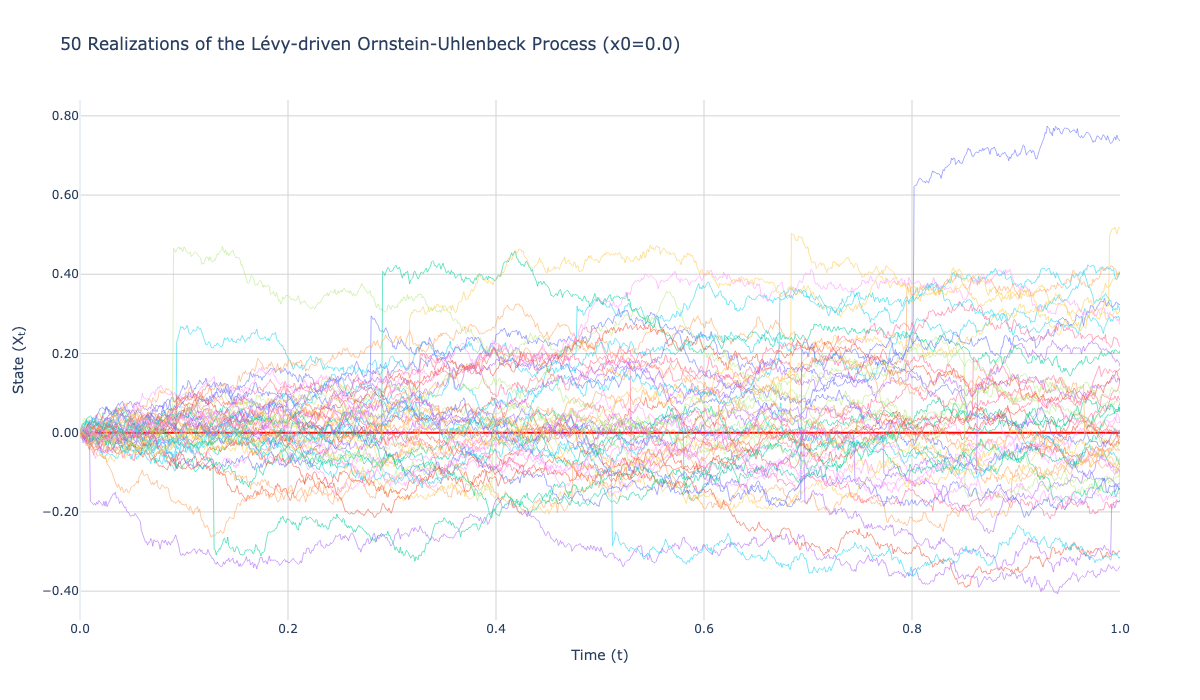
\includegraphics[width=\textwidth]{Figures/levy_ou_process_realizations.png}
    \caption{50 realizations of the Lévy-driven Ornstein-Uhlenbeck process starting from $x_0 = 0$ (the default threshold). The red horizontal line indicates the default boundary $K = 0$. The paths demonstrate both mean-reverting behavior and sudden jump discontinuities that can drive the asset value below the threshold, motivating the extended spatial domain $x \in [-0.5, 2.0]$ used in the PINN training.}
    \label{fig:ou_realizations}
\end{figure}

\begin{figure}[htbp]
    \centering
    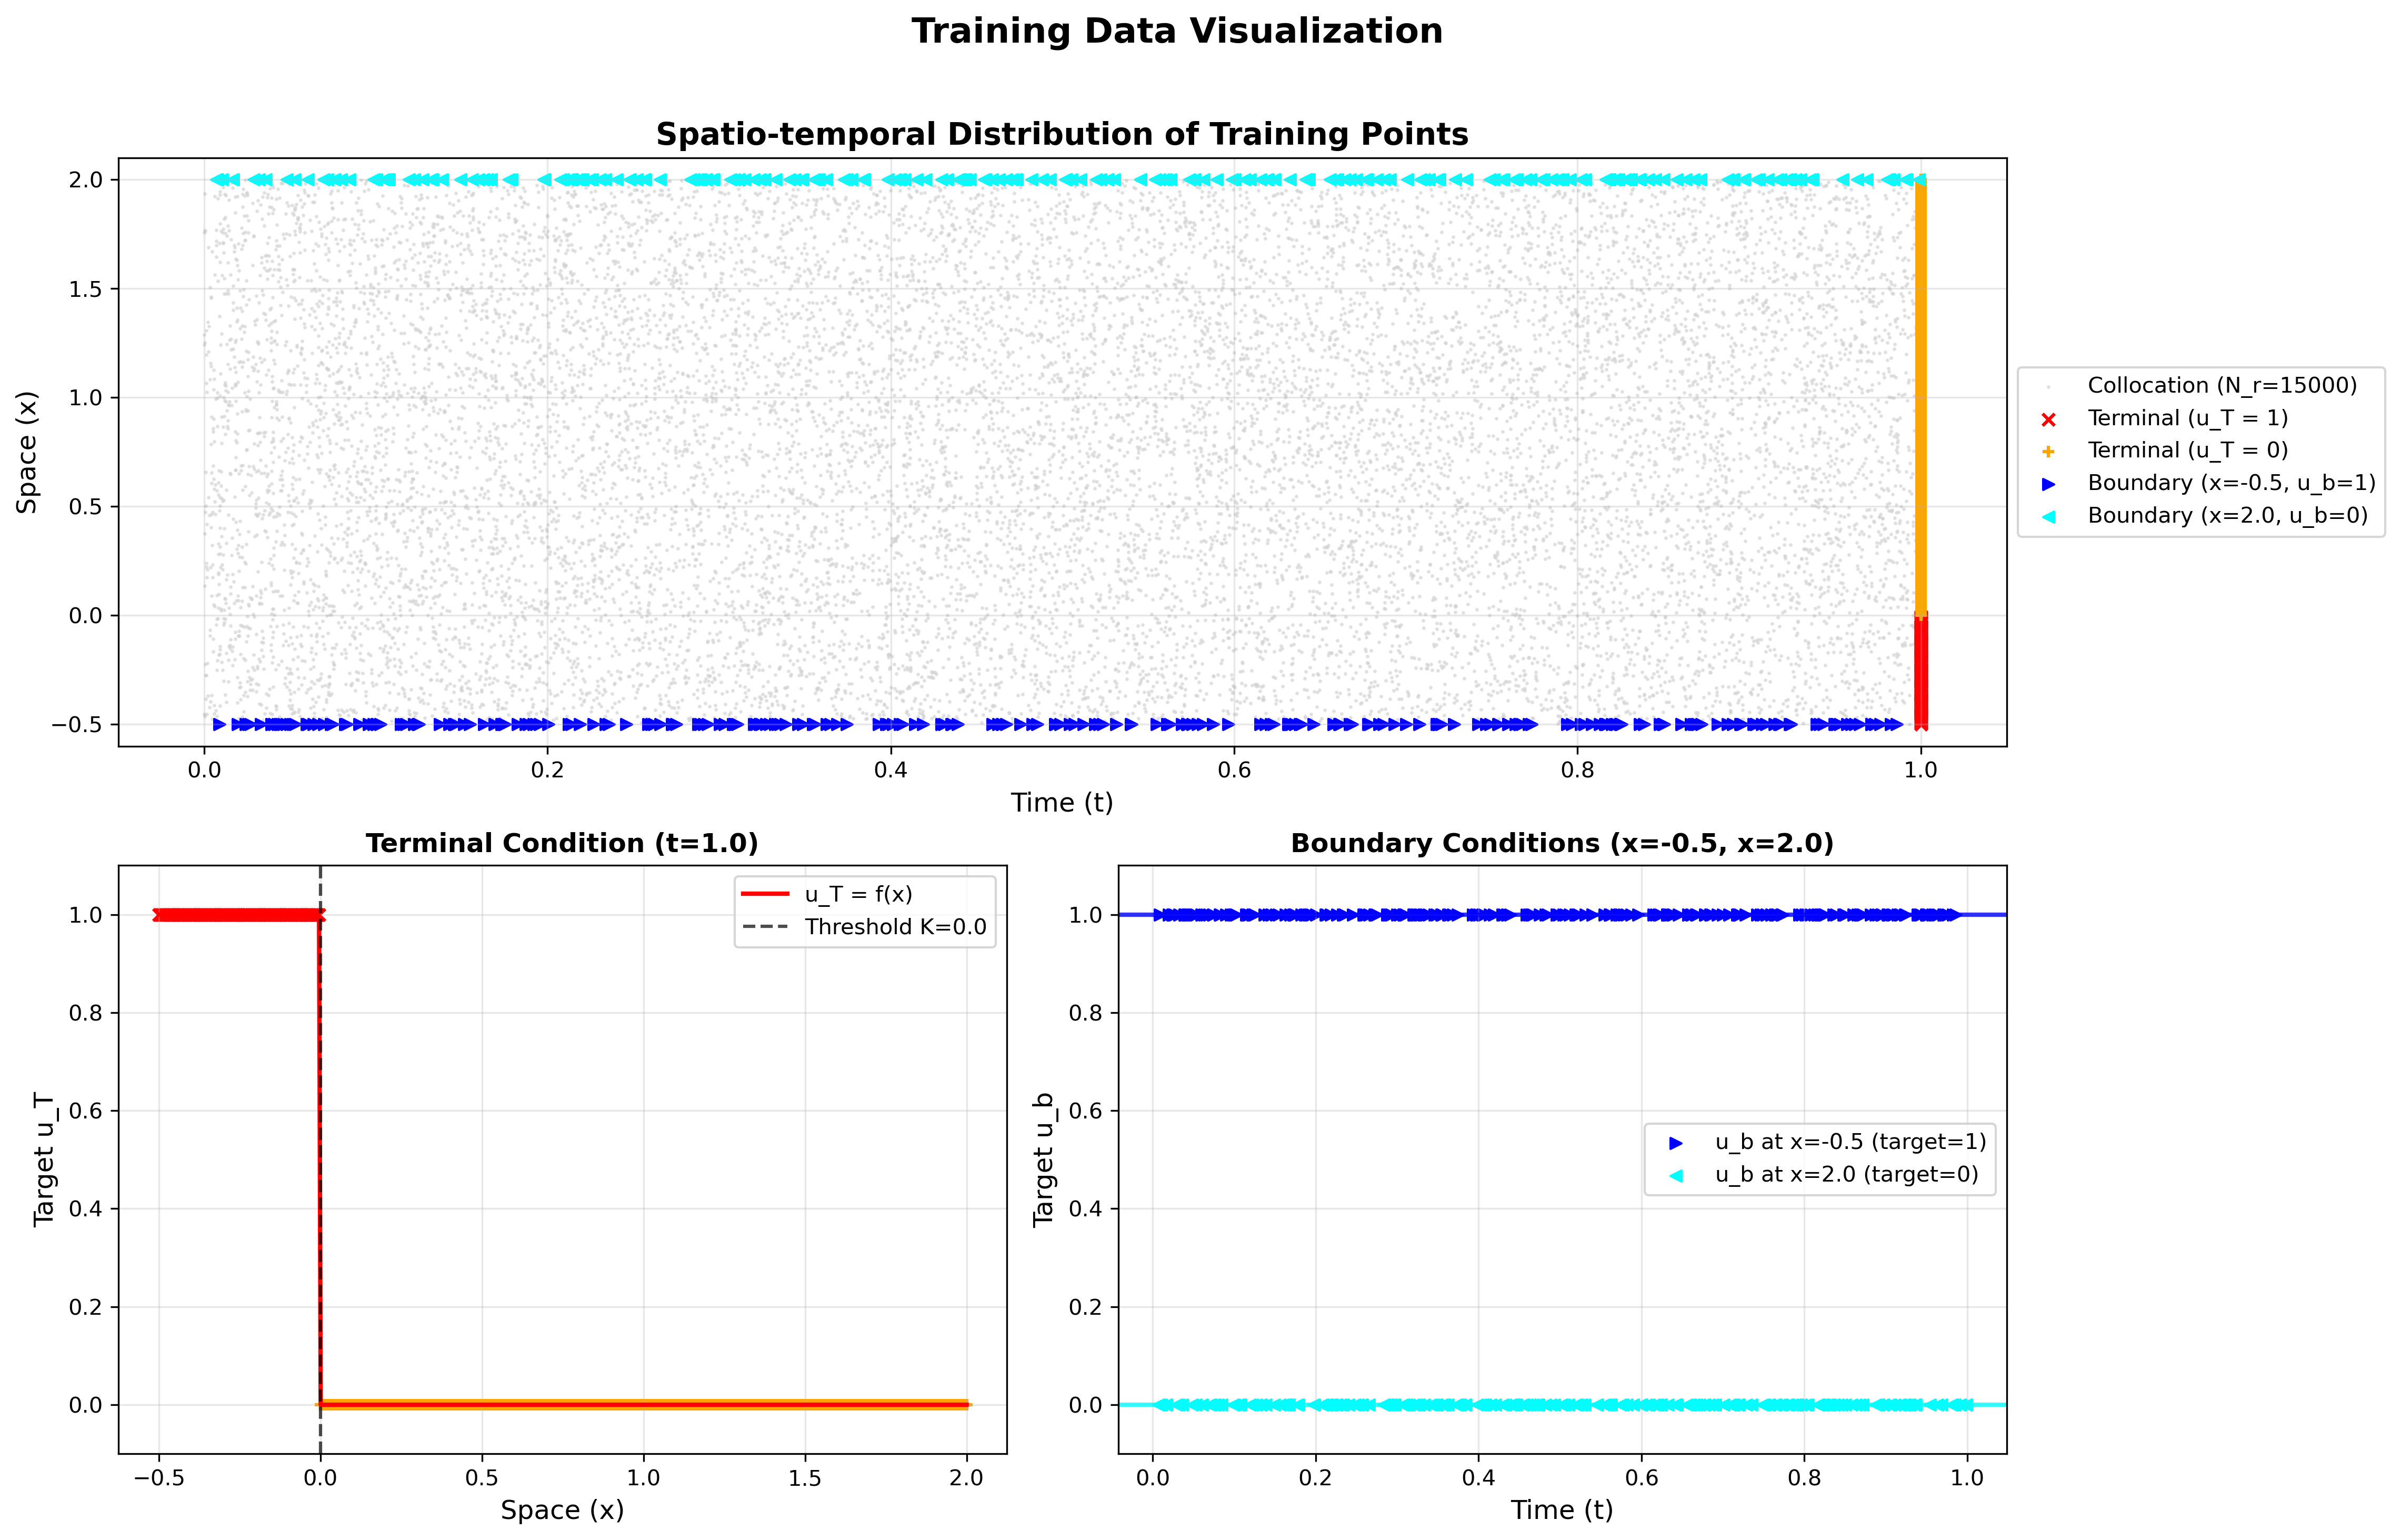
\includegraphics[width=\textwidth]{Figures/training_data_viz_updated.png} % Ensure the image file is accessible
    \caption{Visualization of the training data distribution. Top: Spatio-temporal distribution of collocation, terminal, and boundary points. Bottom-left: Target values for the terminal condition at $t=1.0$. Bottom-right: Target values for the boundary conditions at $x=-0.5$ and $x=2.0$.}
    \label{fig:training_data_viz}
\end{figure}

The training dataset comprises three distinct categories of points:

\begin{itemize}
    \item \textbf{Collocation Points ($N_r$):} As depicted by the dense scatter of light grey dots in the top panel of Figure~\ref{fig:training_data_viz}, $N_r = 15,000$ collocation points are sampled across the interior of the spatio-temporal domain. These points are crucial for enforcing the PIDE residual term in the loss function, ensuring that the learned solution $\hat{\phi}(t,x)$ approximates the governing dynamics of the Lévy-driven Ornstein-Uhlenbeck process throughout the domain. The distribution appears to be uniform random sampling.

    \item \textbf{Terminal Condition Points ($N_T$):} The terminal condition is enforced at $t=1.0$. In the top panel, these points are marked by red 'x' symbols (where the target $u_T=1$) and orange '+' symbols (where the target $u_T=0$). The bottom-left panel provides a clearer view of this condition: $\phi(1.0, x) = u_T$. Specifically, $u_T = 1$ for $x \le 0.0$ and $u_T = 0$ for $x > 0.0$, corresponding to a threshold $K=0.0$. These points ensure that the PINN solution matches the specified final state of the system.

    \item \textbf{Boundary Condition Points ($N_b$):} The conditions at the spatial boundaries $x=-0.5$ and $x=2.0$ are enforced across the entire time interval $t \in [0,1]$. The top panel shows these points as blue right-pointing triangles along $x=-0.5$ (target $u_b=1$) and cyan left-pointing triangles along $x=2.0$ (target $u_b=0$). The bottom-right panel further details these Dirichlet boundary conditions, showing a constant target value of $u_b=1$ at $x=-0.5$ and $u_b=0$ at $x=2.0$ for all $t$. These points constrain the solution behavior at the spatial extremities of the domain.
\end{itemize}

The strategic placement and density of these distinct sets of training points guide the optimization process, enabling the PINN to learn a globally consistent solution that respects both the underlying PIDE and the imposed constraints. The specific quantities $N_T$ and $N_b$ (number of terminal and boundary points respectively) are chosen to provide sufficient constraint without overwhelming the PIDE residual term; in our experiments, these were set to $N_T=500$ and $N_b=500$ (as detailed in Table~\ref{tab:parameters_summary}).

\section{Numerical Results}

\subsection{Training Dynamics and Loss Component Analysis}
\label{sec:training_dynamics}

Before examining the final PINN solution, it is important to analyze the training dynamics and the evolution of different loss components during the optimization process. Figure~\ref{fig:loss_components} illustrates the progression of the total loss and its individual components over 21,000 training epochs.

\begin{figure}[htbp]
    \centering
    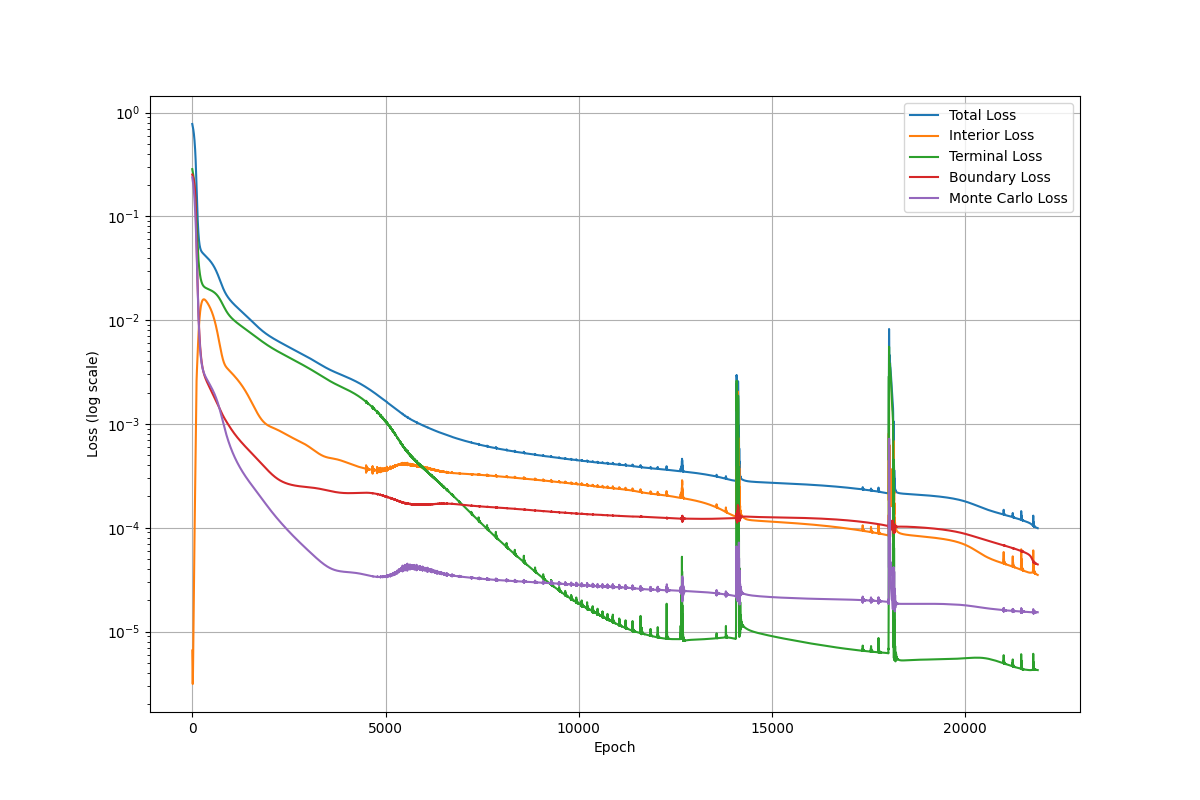
\includegraphics[width=0.9\textwidth]{Figures/loss_components.png}
    \caption{Evolution of loss components during PINN training. The plot shows the decay of total loss (blue) and its constituent components: interior loss from PIDE residual enforcement (orange), terminal condition loss (green), boundary condition loss (red), and Monte Carlo anchor loss (purple). The logarithmic scale reveals the convergence behavior of each component across 21,000 training epochs.}
    \label{fig:loss_components}
\end{figure}

The training dynamics reveal several important characteristics of the PINN optimization process:

\begin{itemize}
    \item \textbf{Rapid Initial Convergence:} All loss components exhibit steep initial decay during the first 1,000 epochs, indicating that the network quickly learns to approximate the basic structure of the solution and satisfy the imposed constraints.
    
    \item \textbf{Interior Loss Dominance:} The interior loss (orange line), corresponding to the PIDE residual enforcement, initially dominates the total loss magnitude. This component represents the network's ability to satisfy the governing integro-differential equation across the computational domain, including the complex jump integral terms approximated via Monte Carlo integration.
    
    \item \textbf{Terminal and Boundary Condition Convergence:} The terminal condition loss (green) and boundary condition loss (red) decrease rapidly and reach very low values (below $10^{-4}$), demonstrating that the network successfully learns to satisfy the prescribed conditions at $t=T$ and the spatial boundaries $x=x_{\min}, x_{\max}$.
    
    \item \textbf{Monte Carlo Anchor Regularization:} The Monte Carlo loss component (purple) provides additional regularization through pre-computed reference solutions at selected points. This component converges to low values and helps guide the overall training process, particularly in regions where the PIDE enforcement alone might be insufficient.
    
    \item \textbf{Fluctuations in Loss Components:} The occasional spikes in individual components (mostly visible in the terminal and boundary losses) suggest that adaptive rebalancing is happening as the optimization explores the parameter space.
\end{itemize}

The successful convergence of all loss components to values below $10^{-4}$ demonstrates the effectiveness of the multi-objective training approach. The balanced reduction across all terms ensures that the final solution simultaneously satisfies the governing PIDE, boundary conditions, terminal conditions, and matches the Monte Carlo reference data. This comprehensive loss reduction is essential for obtaining accurate approximations of the probability of default function.

\subsection{PINN Solution for Probability of Default}
\label{sec:pinn_pd_solution_results} % Changed label slightly
 
The solution to the Partial Integro-Differential Equation (PIDE) governing the Probability of Default (PD) for the Lévy-driven Ornstein-Uhlenbeck process was approximated using a Physics-Informed Neural Network (PINN). The learned solution, denoted by $\hat{\phi}(t, x; \mathbf{\Theta})$, estimates the probability that the process $X_s$ hits or crosses below a predefined threshold $K$ at any time $s \in [t, T]$, given $X_t = x$. Figure~\ref{fig:pinn_levy_ou_pd_solution} visualizes this learned function over the computational domain $(t, x) \in [0, 1] \times [-0.5, 2.0]$.
 
\begin{figure}[htbp]
    \centering
    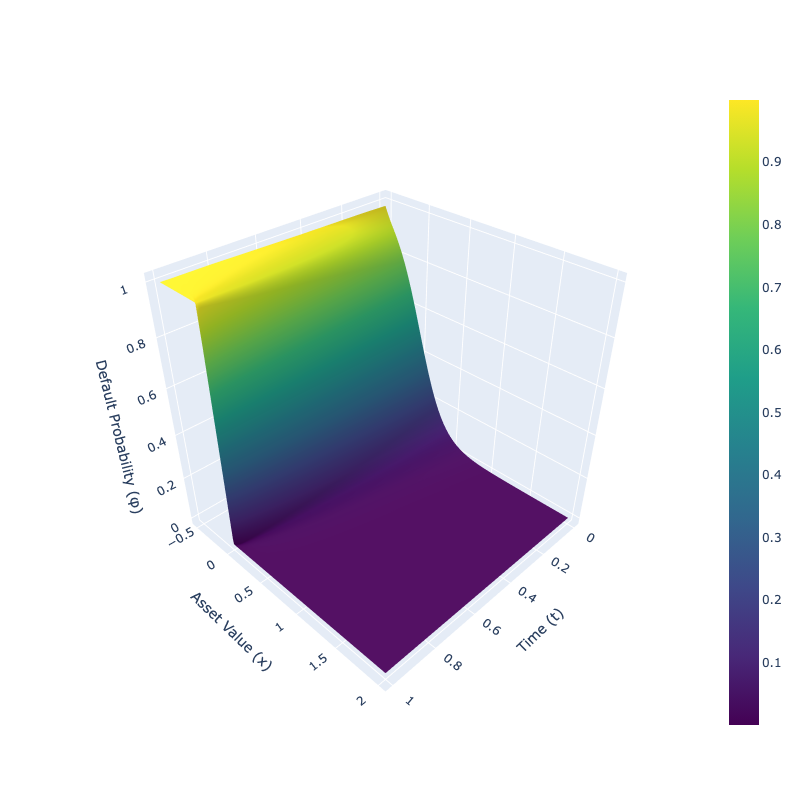
\includegraphics[width=0.8\textwidth]{Figures/pinn_3d_stable_data.png} %<-- REPLACE WITH PATH TO THIS NEW IMAGE
    \caption{Surface plot of the PINN-approximated solution $\hat{\phi}(t, x; \mathbf{\Theta})$ representing the Probability of Default $P(\min_{s \in [t, T]} X_s \le K | X_t = x)$ of a Lévy-driven OU process, with parameters $k=0.3, \theta=0.0, \sigma=0.2, \lambda=1.0, \text{jump\_std}=0.2$, threshold $K=0.0$, final time $T=1.0$, and spatial domain $[-0.5, 2]$.}
    \label{fig:pinn_levy_ou_pd_solution} % Changed label slightly
\end{figure}
 
The plot illustrates the behavior of the Probability of Default as learned by the neural network. The axes represent time $t$, the state variable $x$, and the predicted probability $\hat{\phi}(t, x)$. The learned solution demonstrates good adherence to the imposed boundary and terminal conditions for the PD with threshold $K=0$:
 
\begin{itemize}
    \item \textbf{Terminal Condition ($t=T=1.0$):} The expected condition is $\phi(T, x) = \mathbf{1}_{x \le K}$. For $K=0$, this requires $\phi(T, x) \approx 1$ for $x \le 0$ and $\phi(T, x) \approx 0$ for $x > 0$. The plot shows $\hat{\phi}(1, x)$ is high (close to 1) near $x=0$ and decreases towards 0 for larger $x$, consistent with this condition.
    \item \textbf{Lower Spatial Boundary ($x=x_{min}=-0.5$):} For states well below the threshold ($x=-0.5$), the probability of default should be high, implying $\phi(t, -0.5) = 1$. The plot correctly shows $\hat{\phi}(t, -0.5)$ remains high (close to 1) across the time interval $t \in [0, 1]$.
    \item \textbf{Upper Spatial Boundary ($x=x_{max}=2.0$):} Starting far above the threshold ($x=2.0$) should result in a very low probability of default, implying $\phi(t, 2.0) = 0$. The plot correctly shows $\hat{\phi}(t, 2.0)$ remains close to 0 for all $t \in [0, 1]$.
\end{itemize}
 
The evolution of the solution backward in time (from $t=1$ to $t=0$) exhibits the characteristic smoothing effect due to the diffusive and jump components of the OU process, governed by the backward PIDE. The curve $\hat{\phi}(0, x)$ at the initial time $t=0$ represents the learned probability of defaulting by time $T=1$ as a function of the starting state $x$. As expected, this initial probability is high for states near the default boundary ($x=0$) and decreases as the initial state $x$ increases.
 
The overall smoothness and the consistent adherence to the boundary and terminal conditions demonstrate that the PINN framework has successfully learned a meaningful approximation to the Probability of Default for this Lévy-driven process. This highlights the capability of PINNs to handle the complexities of PIDEs involving jump components in financial applications.

\subsection{PINN Validation Against Monte Carlo Simulations}
\label{sec:pinn_validation}

To validate the accuracy of the PINN-approximated solution, we compare the neural network predictions against independent Monte Carlo estimates of the true default probability. The validation process employs the same Lévy-driven Ornstein-Uhlenbeck simulation framework used to generate Monte Carlo anchor points during training, but with a significantly larger number of simulation paths to ensure statistical reliability.

\textbf{Monte Carlo Validation Methodology:} For each spatial location $x_0$ at a given time $t$, we simulate $N_{\text{MC}} = 10,000$ independent paths of the Lévy-driven OU process starting from $(t, x_0)$ and evolving until the terminal time $T = 1.0$. Each path follows the discrete-time evolution:
\begin{align}
X_{i+1} &= X_i + k(\theta - X_i)\Delta t + \sigma \sqrt{\Delta t} \, \xi_i + J_i \\
\text{where} \quad J_i &= \begin{cases}
Z_i \sim \mathcal{N}(0, \sigma_{\text{jump}}^2) & \text{with probability } \lambda \Delta t \\
0 & \text{otherwise}
\end{cases}
\end{align}
Here, $\xi_i \sim \mathcal{N}(0,1)$ represents the Brownian increments, and $J_i$ captures the compound Poisson jump component. The Monte Carlo estimate of the default probability is then computed as:
$$
\hat{\phi}_{\text{MC}}(t, x_0) = \frac{1}{N_{\text{MC}}} \sum_{j=1}^{N_{\text{MC}}} \mathbf{1}_{\{\min_{s \in [t,T]} X_s^{(j)} \leq K\}}
$$
where $X_s^{(j)}$ denotes the $j$-th simulated path and $\mathbf{1}_{\{\cdot\}}$ is the indicator function for the first hitting time event.

Figure~\ref{fig:pinn_mc_comparison} presents the validation results at two representative time slices: $t = 0.0$ (initial time) and $t = 0.5$ (mid-period). The comparison demonstrates excellent agreement between the PINN predictions (blue lines) and the Monte Carlo estimates (red dots) across the entire spatial domain. The close alignment validates that the PINN has successfully learned to approximate the complex integro-differential equation governing the default probability, including the accurate treatment of the jump integral term through the embedded Monte Carlo integration technique.

\begin{figure}[htbp]
    \centering
    \begin{subfigure}[b]{0.8\textwidth}
        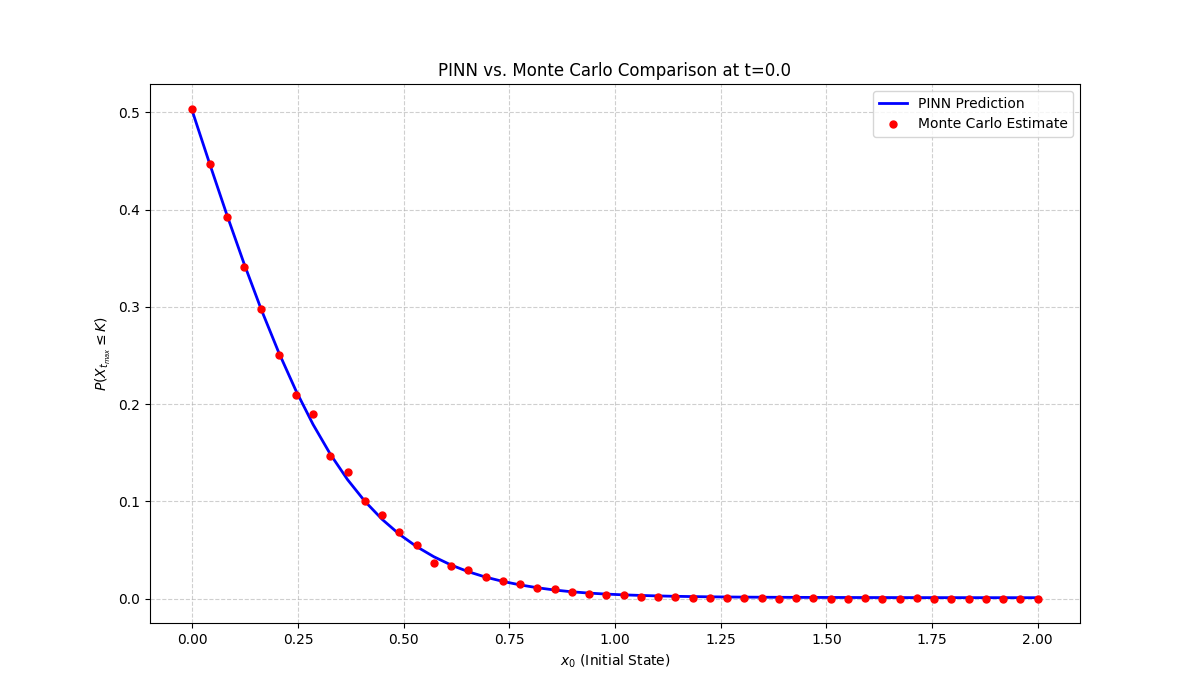
\includegraphics[width=\textwidth]{Figures/pinn_vs_mc_t0.png}
        \caption{Validation at $t = 0.0$}
    \end{subfigure}
    \hfill
    \begin{subfigure}[b]{0.8\textwidth}
        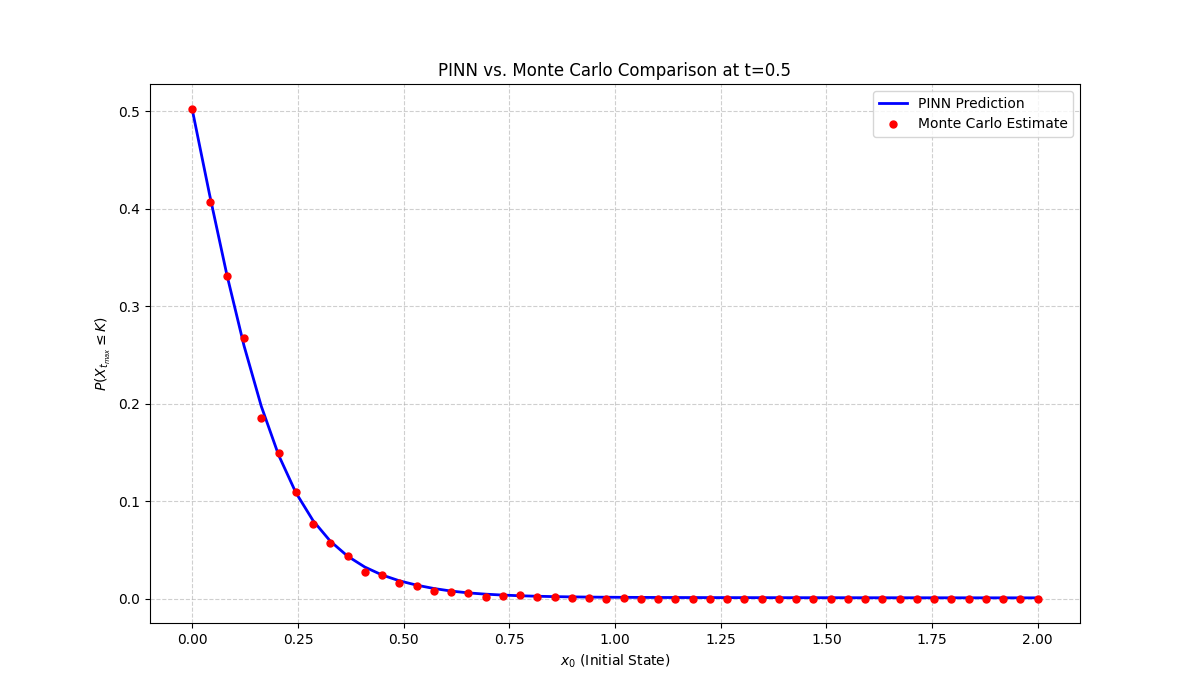
\includegraphics[width=\textwidth]{Figures/pinn_vs_mc_t05.png}
        \caption{Validation at $t = 0.5$}
    \end{subfigure}
    \caption{PINN validation against Monte Carlo simulations. Blue lines show PINN predictions $\hat{\phi}(t,x)$ while red dots represent Monte Carlo estimates $\hat{\phi}_{\text{MC}}(t,x)$ based on 10,000 simulated paths for each spatial point. The excellent agreement demonstrates the accuracy of the PINN approximation across different time horizons and spatial locations.}
    \label{fig:pinn_mc_comparison}
\end{figure}

The validation results confirm that the PINN framework, despite its computational efficiency compared to brute-force Monte Carlo methods, maintains high accuracy in approximating the true default probability function. This demonstrates the practical value of PINNs for solving complex financial PIDEs where traditional numerical methods may be computationally prohibitive.

\subsection{Computational Efficiency: PINN vs. Finite Difference Methods}
\label{sec:computational_efficiency}

A key motivation for employing Physics-Informed Neural Networks over traditional discretization methods lies in their substantial computational efficiency gains during inference. To demonstrate this advantage, we compare our PINN approach with a classical finite difference implementation of the same Lévy-driven OU PIDE problem.

\textbf{Finite Difference Implementation:} We implement a backward-time centered-space (BTCS) implicit finite difference scheme to solve the identical PIDE. The spatial domain is discretized using a uniform grid with spacing $\Delta x$, while the temporal dimension uses uniform time steps $\Delta t$. The continuous PIDE is approximated using second-order central differences for spatial derivatives and backward differences for temporal derivatives:

$$
\frac{\phi_{i}^{n+1} - \phi_{i}^{n}}{\Delta t} + k(\theta - x_i)\frac{\phi_{i+1}^{n+1} - \phi_{i-1}^{n+1}}{2\Delta x} + \frac{\sigma^2}{2}\frac{\phi_{i+1}^{n+1} - 2\phi_{i}^{n+1} + \phi_{i-1}^{n+1}}{(\Delta x)^2} + \mathcal{I}[\phi]_i^{n+1} = 0
$$

where $\phi_{i}^{n}$ represents the discrete solution at spatial point $x_i$ and time level $t_n$. The jump integral term $\mathcal{I}[\phi]_i^{n+1}$ is approximated using a discrete convolution with pre-computed jump probability weights. The resulting linear system is solved at each time step using LU decomposition, requiring matrix inversions that scale as $O(N_x^3)$ for $N_x$ spatial grid points.

\textbf{Computational Requirements:} The finite difference method requires a fine spatial grid ($\Delta x = 0.0037$) and temporal discretization ($\Delta t = 0.001$) to ensure numerical stability and accuracy, resulting in a computational grid of $1000 \times 1000 = 10^6$ points. Each time step involves solving a large sparse linear system, with the total computational time scaling proportionally to the number of time steps.

Figure~\ref{fig:pinn_fd_comparison} presents a side-by-side comparison of the PINN and finite difference solutions, demonstrating excellent visual agreement between the two methods. More importantly, the comparison reveals dramatic computational efficiency differences: the finite difference method requires approximately 98.14 seconds to generate the complete solution, while the trained PINN provides inference across the same domain in approximately 0.0268 seconds, representing a 3,660× speedup (MacBook Air with Apple M2 chip, 16 GB unified memory).

\begin{figure}[htbp]
    \centering
    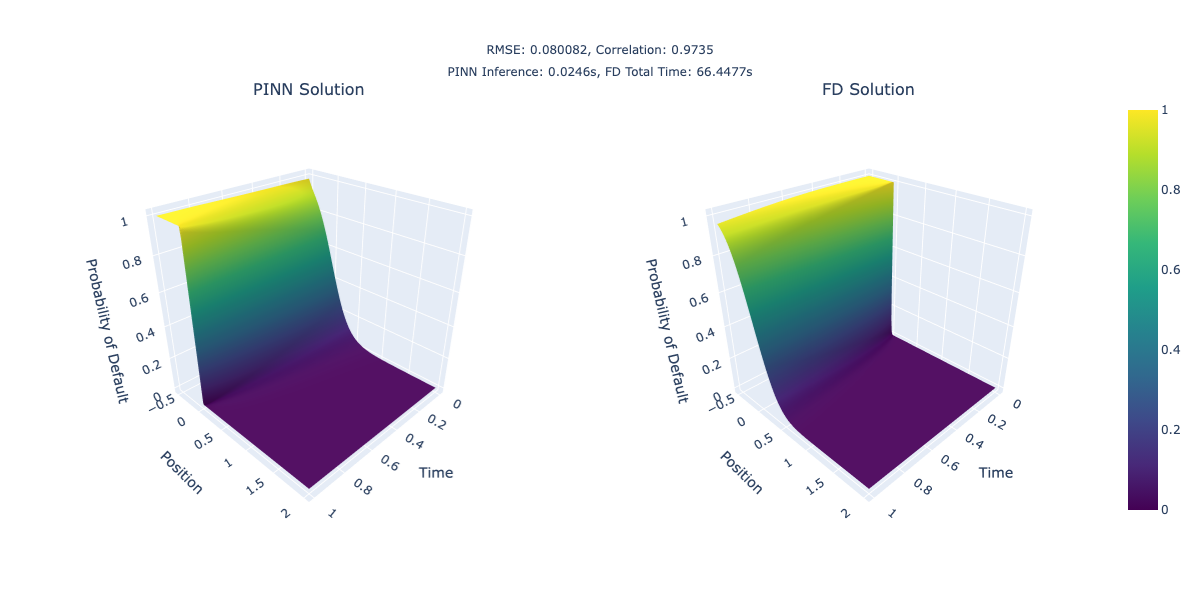
\includegraphics[width=\textwidth]{Figures/comparison_side_by_side.png}
    \caption{Computational efficiency comparison between PINN and finite difference methods. Both solutions show excellent agreement (RMSE: 0.080082, Correlation: 0.9735), but the PINN achieves a remarkable 3,660× speedup in inference time (0.0268s vs 98.14s) while maintaining comparable accuracy. This computational advantage demonstrates the practical value of PINNs for real-time financial applications requiring rapid probability of default calculations.}
    \label{fig:pinn_fd_comparison}
\end{figure}

\textbf{Practical Implications:} This computational efficiency advantage becomes crucial in financial applications where rapid probability of default calculations are required. Consider practical scenarios such as:
\begin{itemize}
    \item \textbf{Real-time Risk Monitoring:} Portfolio risk systems requiring instantaneous updates across thousands of positions
    \item \textbf{Stress Testing:} Monte Carlo simulations requiring millions of default probability evaluations under different market scenarios  
    \item \textbf{High-frequency Trading:} Algorithmic trading systems needing millisecond-level risk assessments
    \item \textbf{Regulatory Reporting:} IFRS 9 expected credit loss calculations across large loan portfolios
\end{itemize}

In such applications, the finite difference approach becomes computationally prohibitive, requiring nearly 100 seconds per calculation. In contrast, the PINN enables real-time evaluation with negligible computational overhead, making sophisticated jump-diffusion models practically viable for production financial systems.

\textbf{Training vs. Inference Trade-off:} While PINN training requires upfront computational investment (40,000 epochs taking several hours), this cost is amortized across millions of subsequent inferences. The trained network becomes a highly efficient "compiled" representation of the PIDE solution, enabling instant evaluation at arbitrary points in the domain without resolving the underlying differential equation. This paradigm shift from "solve each time" (finite difference) to "solve once, evaluate many times" (PINN) represents the fundamental computational advantage driving PINN adoption in quantitative finance.

\section{Conclusion}
\label{sec:exp_conclusion}

This chapter presented a comprehensive experimental framework for applying Physics-Informed Neural Networks to solve partial integro-differential equations arising in credit risk modeling. We demonstrated how PINNs can effectively approximate the probability of default for Lévy-driven Ornstein-Uhlenbeck processes, combining the mathematical rigor of traditional numerical methods with the computational efficiency of modern machine learning.

The experimental results reveal three key achievements. First, the PINN successfully learned to satisfy the complex PIDE governing jump-diffusion processes, as evidenced by the close agreement with Monte Carlo simulations across different time horizons and spatial locations. Second, the method achieved remarkable computational efficiency, providing inference times of 0.0268 seconds compared to 98.14 seconds for traditional finite difference methods (a speedup factor of approximately 3,660). Third, the approach demonstrated robust handling of boundary conditions and jump discontinuities through careful domain extension and training data design.

Additionally, the validation against independent Monte Carlo simulations confirmed the reliability of the learned solution, while the comparison with finite difference methods highlighted the practical advantages of the PINN approach for real-time financial applications.

These results establish PINNs as a viable alternative to traditional numerical methods for solving financial PIDEs, particularly in scenarios requiring rapid evaluation of probability of default calculations across varying market conditions and portfolio compositions.

\chapter{Conclusions and Future Directions}
\label{ch:conclusions}

\section{General Conclusions}

This thesis investigated the application of Physics-Informed Neural Networks for solving partial integro-differential equations with particular focus on estimating probabilities of default for Lévy-driven stochastic processes. This work addresses a fundamental challenge in quantitative finance: the need for computationally efficient methods to solve complex mathematical models that capture both continuous market dynamics and sudden jump events.

The primary aim of this work lies in demonstrating that PINNs can effectively replace traditional numerical methods for solving financial PIDEs while providing substantial computational advantages. We showed that neural networks can learn the underlying physics of jump-diffusion processes without requiring explicit discretization of the governing equations. This further motivates a paradigm shift from conventional approaches that rely on finite difference or finite element methods.

Our experimental results reveal several important findings. First, the fidelity of the solution from the PINN approach was validated against Monte Carlo simulations for the Lévy-driven OU process. Second, the method delivered computational speedups of over three orders of magnitude compared to traditional finite difference schemes. These efficiency gains are particularly valuable in practical applications where real-time risk assessment is critical, such as algorithmic trading, portfolio optimization, and regulatory stress testing.

From a dynamic systems modeling perspective, this work contributes to the broader application of physics-informed neural networks for solving integro-differential equations that govern complex stochastic processes. The methodology developed here extends beyond financial applications to any dynamic system characterized by both continuous evolution and discontinuous jump events. The ability to efficiently approximate solutions to PIDEs with non-local operators demonstrates the potential for PINNs to address a wider class of mathematical models that traditional numerical methods struggle to handle in real-time applications.

\section{Limitations and Future Research Directions}

While this work demonstrates the effectiveness of PINNs for solving financial PIDEs, two key areas warrant further investigation to enhance the methodology's robustness and applicability.

\subsection{Advanced Loss Function Regularization}

The Monte Carlo anchor loss component proved effective in guiding the PINN training process by providing reference solutions at selected points. However, the current implementation uses fixed anchor points throughout training, which may lead the network to memorize specific noise patterns rather than learning the underlying mathematical structure. Future research should explore dynamic regularization strategies where Monte Carlo anchor points are regenerated every few training epochs. This approach would prevent the model from overfitting to particular realizations while maintaining the beneficial regularization effect. The regeneration frequency and sampling strategy for new anchor points present interesting optimization challenges that could significantly improve solution quality and generalization capabilities.

Additionally, investigating adaptive weighting \cite{wang2025simulating} schemes for different loss components based on their convergence rates could improve training stability. The development of physics-informed regularization terms that exploit known properties of the underlying stochastic processes, such as monotonicity constraints or asymptotic behavior, offers another promising direction for enhancing solution accuracy.

\subsection{Multi-Dimensional PIDEs for Multi-Asset Models}

Real-world financial applications frequently involve portfolios of multiple correlated assets, requiring the solution of high-dimensional PIDEs with cross-asset dependencies. Extending the current framework to handle systems of coupled PIDEs represents a critical next step for practical implementation. The challenge lies in efficiently handling the curse of dimensionality while maintaining computational advantages over traditional methods.

Future work should investigate domain decomposition strategies, where high-dimensional problems are broken into manageable sub-problems, and explore specialized neural network architectures designed for multi-asset scenarios. The correlation structure between assets introduces additional complexity in both the jump integral terms and the boundary condition specifications. Developing efficient sampling strategies for multi-dimensional Monte Carlo integration and investigating the scalability of the approach as the number of assets increases will be essential for real-world portfolio applications.

\cleardoublepage
\bibliographystyle{plain}
\bibliography{thesis_references}

\end{document}